\documentclass[10pt]{article}

% ============================================================
% PACKAGES
% ============================================================

\usepackage[a4paper,margin=0.65in]{geometry}
\usepackage{amsmath,amssymb}
\usepackage{graphicx}
\usepackage{booktabs}
\usepackage{array}
\usepackage{float}
\usepackage{hyperref}
\usepackage{enumitem}
\usepackage{xcolor}
\usepackage{tikz}
\usepackage{multirow}
\usepackage{caption}
\usepackage{subcaption}

\usetikzlibrary{
positioning,
arrows.meta,
shapes.geometric,
fit,
calc
}

% ============================================================
% FORMATTING
% ============================================================

\setlist{nosep,leftmargin=*}
\renewcommand{\arraystretch}{1.2}
\setlength{\parindent}{0pt}
\setlength{\parskip}{2pt}

\hypersetup{
    colorlinks=true,
    linkcolor=blue,
    urlcolor=blue,
    citecolor=blue
}

% ============================================================
% TIKZ STYLES
% ============================================================

\tikzset{
block/.style={
draw,
rounded corners,
minimum width=1.55cm,
minimum height=0.60cm,
align=center,
fill=blue!10,
font=\scriptsize
},
attn/.style={
draw,
rounded corners,
minimum width=1.55cm,
minimum height=0.60cm,
align=center,
fill=green!12,
font=\scriptsize
},
arrow/.style={
-{Latex[length=2mm]},
thin
}
}

% ============================================================
% DOCUMENT
% ============================================================

\begin{document}

% ============================================================
% TITLE
% ============================================================

\begin{center}

{\large\textbf{Shiv Nadar University Chennai}}\\[2mm]

{\normalsize\textbf{CS3807 -- Deep Learning Laboratory}}\\[2mm]

{\large\textbf{Experiments 8, 9}}\\[1mm]

{\normalsize
\textbf{
Effect of Attention Type and Attention Position\\
in a Pretrained ResNet50
}}\\[4mm]
Ankith U Davey\hspace{1.2em}24011101004

\end{center}

\vspace{3mm}

% ============================================================
% COURSE DETAILS
% ============================================================

\begin{center}
\begin{tabular}{|p{3.5cm}|p{8.7cm}|p{2.1cm}|}
\hline
\textbf{Degree \& Branch}
&
B.Tech Artificial Intelligence \& Data Science
&
Semester V
\\
\hline

\textbf{Subject Code \& Name}
&
CS3807 -- Deep Learning Laboratory
&
AY: 2026--27
\\
\hline

\end{tabular}
\end{center}

% ============================================================
\section*{1. Objective}
% ============================================================

The objective of this experiment is to understand how different attention
mechanisms modify a pretrained convolutional neural network and how the
\textbf{position at which attention is inserted} influences image
classification performance.

A single pretrained architecture,

\[
\boxed{\text{ResNet50 pretrained on ImageNet}}
\]

is used throughout the experiment.

\begin{itemize}

\item Channel attention;

\item Spatial attention;

\item Sequential channel--spatial attention;

\item Lightweight self-attention;

\item Different positions for inserting attention within ResNet50;

\item Single-stage and multi-stage attention;

\item Attention ordering;

\item Additional established attention mechanisms; and

\item Qualitative interpretation using internal attention maps and Grad-CAM.

\end{itemize}

The experiment emphasizes that the effectiveness of attention depends not
only on the attention mechanism itself, but also on the characteristics of
the feature representation on which it operates.

% ============================================================
\section*{2. Learning Outcomes}
% ============================================================

\begin{enumerate}

\item Explain the stage-wise architecture of a pretrained ResNet50;

\item Distinguish early, intermediate, and late convolutional features;

\item Explain the motivation behind attention mechanisms;

\item Implement channel attention;

\item Implement spatial attention;

\item Implement sequential channel--spatial attention;

\item Implement a lightweight self-attention mechanism;

\item Insert an attention module at different stages of a pretrained network;

\item Analyze the influence of attention position;

\item Compare different attention mechanisms under a controlled experimental
protocol;

\item Analyze classification accuracy and class-wise performance;

\item Visualize internal attention maps;

\item Generate Grad-CAM explanations;

\item Distinguish an internal attention map from a post-hoc explanation map;

\item Analyze accuracy--complexity trade-offs; and

\item Perform controlled ablation studies.

\end{enumerate}

% ============================================================
\section*{3. Dataset}
% ============================================================

\textbf{Recommended Dataset: TensorFlow Flowers (\texttt{tf\_flowers})}

The TensorFlow Flowers dataset contains natural RGB flower images belonging
to five classes:

\begin{center}
\texttt{daisy},
\quad
\texttt{dandelion},
\quad
\texttt{roses},
\quad
\texttt{sunflowers},
\quad
\texttt{tulips}.
\end{center}

The images contain variations in:

\begin{itemize}

\item scale;

\item viewpoint;

\item illumination;

\item background clutter;

\item flower size;

\item color;

\item texture; and

\item object location.

\end{itemize}

These variations make the dataset suitable for studying the behavior of
attention mechanisms.

% ============================================================
\subsection*{3.1 Image Preprocessing}
% ============================================================

Resize every input image to

\[
224\times224\times3.
\]

The image should be preprocessed using the preprocessing procedure expected
by the ImageNet-pretrained ResNet50.

Suitable data augmentation may include:

\begin{itemize}

\item random horizontal flipping;

\item small rotations;

\item random zoom;

\item random translation; and

\item mild contrast variation.

\end{itemize}

The same augmentation strategy must be maintained for all model comparisons.

% ============================================================
\subsection*{3.2 Dataset Split}
% ============================================================

Use the same training, validation, and testing split for every experiment:

\[
\boxed{
70\% : 15\% : 15\%
}
\]

for

\[
\text{Training : Validation : Testing}.
\]

The exact same samples should be retained in each subset for all ablation
experiments.

This is necessary to ensure that differences in performance are caused by
changes in the model rather than changes in the dataset split.

The dataset has 3670 images. The split gave 2569 training, 550 validation and 551 test images, and the same split was used for every run. Dandelion has the most images (898) and daisy the fewest (633), so the classes are only mildly imbalanced. Macro F1 is still reported next to accuracy so that the smaller classes count equally.

\begin{table}[H]
\centering
\caption{Class-wise image counts in the fixed split.}
\begin{tabular}{|l|c|c|c|c|}
\hline
\textbf{Class} & \textbf{Train} & \textbf{Validation} & \textbf{Test} & \textbf{Total}\\
\hline
dandelion & 629 & 134 & 135 & 898\\
\hline
daisy & 443 & 95 & 95 & 633\\
\hline
tulips & 559 & 120 & 120 & 799\\
\hline
sunflowers & 489 & 105 & 105 & 699\\
\hline
roses & 449 & 96 & 96 & 641\\
\hline
\textbf{Total} & 2569 & 550 & 551 & 3670\\
\hline
\end{tabular}
\end{table}

\begin{figure}[!htbp]
\centering
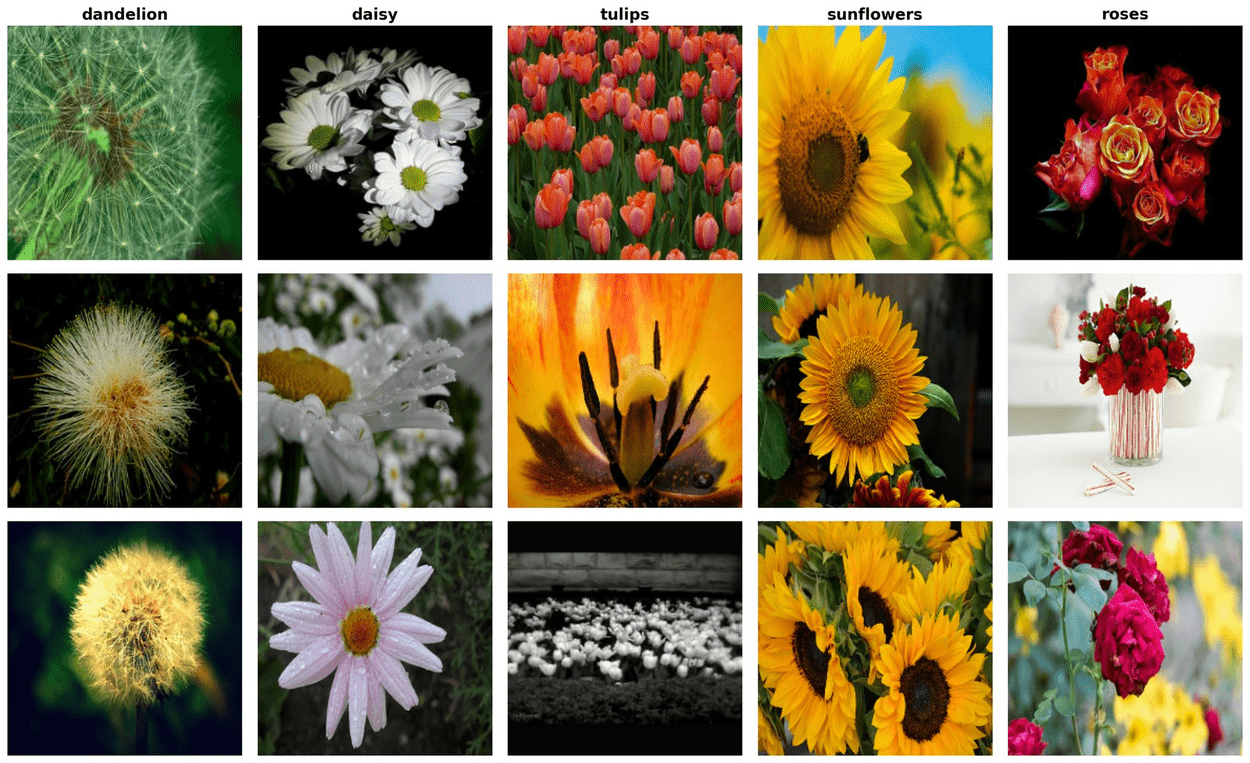
\includegraphics[width=0.92\textwidth]{plots/01_sample_images.png}
\caption{Sample training images from the five classes (columns: dandelion, daisy, tulips, sunflowers, roses).}
\label{fig:samples}
\end{figure}
The images differ a lot in scale, background and lighting. Some flowers fill the whole frame while others are small with grass or leaves around them. Tulips and roses are both red or pink in many of the samples, so they are expected to be the hardest pair, and the confusion matrices later confirm this.

% ============================================================
\section*{4. Source Code}
% ============================================================

The complete code (split, models, training, evaluation, plots and tables) is available at:

{\small\url{https://github.com/Ankith-Davey/Deep-Learning-Lab-Ankith-24011101004/tree/main/Lab%208%20%26%209}}

% ============================================================
\section*{5. Pretrained Architecture: ResNet50}
% ============================================================

ResNet50 pretrained using ImageNet is used as the
\textbf{only backbone architecture} in this experiment.

For an input image

\[
I\in\mathbb{R}^{224\times224\times3},
\]

the major ResNet50 stages produce approximately the following feature
dimensions:

\begin{center}

\begin{tabular}{|l|c|c|}
\hline
\textbf{ResNet50 Stage}
&
\textbf{Spatial Resolution}
&
\textbf{Channels}
\\
\hline

Stem + MaxPool
&
$56\times56$
&
64
\\
\hline

conv2\_x
&
$56\times56$
&
256
\\
\hline

conv3\_x
&
$28\times28$
&
512
\\
\hline

conv4\_x
&
$14\times14$
&
1024
\\
\hline

conv5\_x
&
$7\times7$
&
2048
\\
\hline

\end{tabular}

\end{center}

As the network becomes deeper:

\[
\boxed{
\text{Spatial Resolution}\downarrow
}
\]

while

\[
\boxed{
\text{Feature Channels}\uparrow
}
\]

and the representation generally progresses from low-level visual
information toward higher-level semantic information.

% ============================================================
\section*{6. Understanding ResNet50 Feature Hierarchy}
% ============================================================

The approximate interpretation of different stages is:

\begin{itemize}

\item \textbf{Early features:}
edges, colors, orientations, boundaries, and simple textures.

\item \textbf{Intermediate features:}
local patterns, repeated structures, flower parts, petal arrangements, and
shape information.

\item \textbf{Late features:}
high-level object structures and class-discriminative semantic information.

\end{itemize}

Therefore, the same attention mechanism may produce different behavior when
inserted at different locations.

% ============================================================
\section*{7. Why Attention Position Matters}
% ============================================================

Attention is not independent of the features on which it operates.

Suppose an attention module receives

\[
F\in\mathbb{R}^{H\times W\times C}.
\]

The values of

\[
H,\qquad W,\qquad C
\]

and the semantic meaning of the feature tensor change significantly with
network depth.

Therefore:

\begin{itemize}

\item \textbf{early-stage attention} operates on high-resolution,
low-level visual information;

\item \textbf{middle-stage attention} operates on intermediate features
containing both spatial and semantic information; and

\item \textbf{late-stage attention} operates on low-resolution,
high-level semantic representations.

\end{itemize}

% ============================================================
\section*{8. Candidate Attention Positions}
% ============================================================

\[
P_1:
\text{ after conv2\_x},
\]

\[
P_2:
\text{ after conv3\_x},
\]

\[
P_3:
\text{ after conv4\_x},
\]

\[
P_4:
\text{ after conv5\_x}.
\]

The corresponding feature dimensions are:

\begin{center}

\begin{tabular}{|c|c|c|c|}
\hline

\textbf{Position}
&
\textbf{Location}
&
\textbf{Resolution}
&
\textbf{Channels}
\\
\hline

$P_1$
&
After conv2\_x
&
$56\times56$
&
256
\\
\hline

$P_2$
&
After conv3\_x
&
$28\times28$
&
512
\\
\hline

$P_3$
&
After conv4\_x
&
$14\times14$
&
1024
\\
\hline

$P_4$
&
After conv5\_x
&
$7\times7$
&
2048
\\
\hline

\end{tabular}

\end{center}

% ============================================================
\section*{9. Baseline Model}
% ============================================================

The baseline is the pretrained ResNet50 without any additional attention
mechanism.

\begin{center}

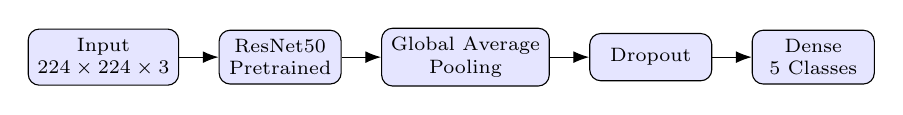
\begin{tikzpicture}[node distance=5mm]

\node[block] (a)
{Input\\$224\times224\times3$};

\node[block,right=of a] (b)
{ResNet50\\Pretrained};

\node[block,right=of b] (c)
{Global Average\\Pooling};

\node[block,right=of c] (d)
{Dropout};

\node[block,right=of d] (e)
{Dense\\5 Classes};

\foreach \x/\y in {a/b,b/c,c/d,d/e}
\draw[arrow] (\x)--(\y);

\end{tikzpicture}

\end{center}

The baseline establishes the reference performance against which the
attention-based models are compared.

% ============================================================
\section*{10. Channel Attention}
% ============================================================

Consider a feature tensor

\[
F\in\mathbb{R}^{H\times W\times C}.
\]

Channel attention determines the relative importance of different feature
channels.

Global average pooling is first used to generate a channel descriptor:

\[
z_c
=
\frac{1}{HW}
\sum_{i=1}^{H}
\sum_{j=1}^{W}
F(i,j,c).
\]

Thus,

\[
z\in\mathbb{R}^{C}.
\]

The channel descriptor is transformed using two learnable transformations:

\[
M_c(F)
=
\sigma
\left(
W_2
\delta
\left(
W_1z
\right)
\right),
\]

where:

\begin{itemize}

\item $\delta(\cdot)$ denotes a nonlinear activation such as ReLU;

\item $\sigma(\cdot)$ denotes the sigmoid activation;

\item $W_1$ reduces the channel representation; and

\item $W_2$ restores the channel dimension.

\end{itemize}

The refined feature tensor is:

\[
F_c
=
F\odot M_c(F).
\]

Channel attention attempts to answer:

\[
\boxed{\text{Which feature channels are important?}}
\]

A reduction ratio of

\[
r=16
\]

may be used as the default setting throughout the laboratory experiment.

The reduction ratio need not be treated as a separate mandatory ablation.

% ============================================================
\section*{11. Spatial Attention}
% ============================================================

Spatial attention determines the spatial regions that should receive greater
importance.

For the input feature tensor

\[
F\in\mathbb{R}^{H\times W\times C},
\]

compute average pooling across channels:

\[
F_{\mathrm{avg}}
=
\operatorname{Mean}_{c}(F),
\]

and maximum pooling across channels:

\[
F_{\mathrm{max}}
=
\operatorname{Max}_{c}(F).
\]

Both tensors have dimensions

\[
H\times W\times1.
\]

Concatenate them:

\[
F_s
=
[
F_{\mathrm{avg}}
\Vert
F_{\mathrm{max}}
].
\]

The spatial attention map is then computed as

\[
M_s(F)
=
\sigma
\left(
\operatorname{Conv}_{7\times7}(F_s)
\right).
\]

Therefore,

\[
M_s(F)
\in
\mathbb{R}^{H\times W\times1}.
\]

The spatially refined feature is

\[
F_s'
=
F\odot M_s(F).
\]

Spatial attention answers:

\[
\boxed{\text{Which spatial locations are important?}}
\]

% ============================================================
\section*{12. Sequential Channel--Spatial Attention}
% ============================================================

Channel and spatial attention can be sequentially applied.

First,

\[
F_c
=
M_c(F)\odot F.
\]

Then,

\[
F_{cs}
=
M_s(F_c)\odot F_c.
\]

The overall structure becomes:

\[
\boxed{
F
\rightarrow
\text{Channel Attention}
\rightarrow
\text{Spatial Attention}
\rightarrow
F_{cs}
}
\]

This arrangement first determines

\[
\text{``what is important''}
\]

and then determines

\[
\text{``where it is important.''}
\]

A simplified diagram is shown below.

\begin{center}

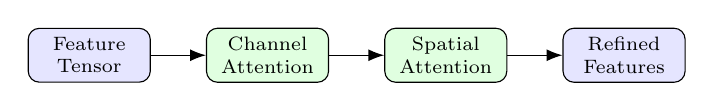
\begin{tikzpicture}[node distance=7mm]

\node[block] (a)
{Feature\\Tensor};

\node[attn,right=of a] (b)
{Channel\\Attention};

\node[attn,right=of b] (c)
{Spatial\\Attention};

\node[block,right=of c] (d)
{Refined\\Features};

\draw[arrow] (a)--(b);
\draw[arrow] (b)--(c);
\draw[arrow] (c)--(d);

\end{tikzpicture}

\end{center}

% ============================================================
\section*{13. Self-Attention}
% ============================================================

Self-attention allows spatial locations to interact directly with other
spatial locations.

For

\[
F\in\mathbb{R}^{H\times W\times C},
\]

flatten the spatial dimensions:

\[
X\in\mathbb{R}^{N\times C},
\]

where

\[
N=HW.
\]

Generate the query, key, and value matrices:

\[
Q=XW_Q,
\]

\[
K=XW_K,
\]

and

\[
V=XW_V.
\]

The attention matrix is

\[
A
=
\operatorname{softmax}
\left(
\frac{QK^T}{\sqrt{d}}
\right),
\]

where $d$ is the dimension of the query/key representation.

The attended output is

\[
Y=AV.
\]

After reshaping the output back to the original spatial structure, a residual
formulation may be used:

\[
F_{\mathrm{SA}}
=
F
+
\gamma
\operatorname{reshape}(Y),
\]

where $\gamma$ is a learnable scaling parameter.

Self-attention attempts to answer:

\[
\boxed{
\text{Which spatial features are related to other spatial features?}
}
\]

Since the attention matrix has dimension approximately

\[
N\times N,
\]

its computational requirements increase rapidly as

\[
N=HW
\]

increases.

Therefore, self-attention should preferably be introduced at

\[
P_3
\]

or

\[
P_4.
\]

% ============================================================
\section*{14. Inserting Attention into ResNet50}
% ============================================================

For any selected stage $P_k$, the network structure can be written as

\[
\text{Previous ResNet Stage}
\rightarrow
\text{Attention}
\rightarrow
\text{Next ResNet Stage}.
\]

For example, attention inserted after conv4\_x gives:

\[
\boxed{
\text{conv4\_x}
\rightarrow
\text{Attention}
\rightarrow
\text{conv5\_x}
}
\]

For channel--spatial attention:

\[
\boxed{
\text{conv4\_x}
\rightarrow
\text{Channel Attention}
\rightarrow
\text{Spatial Attention}
\rightarrow
\text{conv5\_x}
}
\]

Attention should not unintentionally modify the spatial or channel
dimensions unless the selected mechanism explicitly requires such a
transformation.

The attention modules did not change the feature size at any position, so the next ResNet50 stage gets the shape it expects and its pretrained weights still apply. The parameters added by Channel+Spatial grow with the channel count, from 8563 at $P_1$ to 526563 at $P_4$. This is about four times more each time the channels double.

\begin{table}[H]
\centering
\caption{Input and output feature dimensions of the attention block at each position.}
\begin{tabular}{|c|l|c|c|}
\hline
\textbf{Position} & \textbf{Location} & \textbf{Input $(H,W,C)$} & \textbf{Output $(H,W,C)$}\\
\hline
$P_1$ & after conv2\_x & $(56,56,256)$ & $(56,56,256)$\\
\hline
$P_2$ & after conv3\_x & $(28,28,512)$ & $(28,28,512)$\\
\hline
$P_3$ & after conv4\_x & $(14,14,1024)$ & $(14,14,1024)$\\
\hline
$P_4$ & after conv5\_x & $(7,7,2048)$ & $(7,7,2048)$\\
\hline
\end{tabular}
\end{table}

% ============================================================
\section*{15. Main Experiment 1: Attention-Type Ablation}
% ============================================================

The first experiment studies the effect of different types of attention.

Fix the attention position at

\[
\boxed{
P_3=\text{after conv4\_x}
}
\]

for all models.

Compare the following:

\begin{center}
\begin{tabular}{|l|c|c|c|}
\hline
\textbf{Model} & \textbf{Channel} & \textbf{Spatial} & \textbf{Self-Attention} \\
\hline
A0: Baseline ResNet50 & \textcolor{gray}{--} & \textcolor{gray}{--} & \textcolor{gray}{--} \\
\hline
A1: Channel Attention & $\checkmark$ & \textcolor{gray}{--} & \textcolor{gray}{--} \\
\hline
A2: Spatial Attention & \textcolor{gray}{--} & $\checkmark$ & \textcolor{gray}{--} \\
\hline
A3: Channel+Spatial & $\checkmark$ & $\checkmark$ & \textcolor{gray}{--} \\
\hline
A4: Self-Attention & \textcolor{gray}{--} & \textcolor{gray}{--} & $\checkmark$ \\
\hline
A5: Combined Attention & $\checkmark$ & $\checkmark$ & $\checkmark$ \\
\hline
\end{tabular}
\end{center}

This experiment investigates:

\[
\boxed{
\text{How does attention type affect model performance?}
}
\]

\begin{table}[H]
\centering
\caption{Attention-type ablation at $P_3$ (after conv4\_x). Inference time is in ms per image (batch of 32).}
\label{tab:type}
\resizebox{\textwidth}{!}{
\begin{tabular}{|l|c|c|c|c|c|c|c|r|c|}
\hline
\textbf{Model} & \textbf{Position} & \textbf{Train Acc (\%)} & \textbf{Val Acc (\%)} & \textbf{Test Acc (\%)} & \textbf{Precision (\%)} & \textbf{Recall (\%)} & \textbf{Macro F1 (\%)} & \textbf{Parameters} & \textbf{Inf. Time (ms)} \\
\hline
A0: Baseline & -- & 99.42 & 93.27 & 92.74 & 93.08 & 92.47 & 92.50 & 23\,597\,957 & 4.55 \\
\hline
A1: Channel & P3 & 99.07 & 93.45 & 92.56 & 92.81 & 92.44 & 92.44 & 23\,730\,117 & 4.47 \\
\hline
A2: Spatial & P3 & 98.91 & 93.82 & 91.65 & 91.87 & 91.25 & 91.51 & 23\,598\,056 & 4.50 \\
\hline
A3: Channel+Spatial & P3 & 98.95 & 91.82 & 91.11 & 91.98 & 90.87 & 90.91 & 23\,730\,216 & 4.63 \\
\hline
A4: Self-Attention & P3 & 98.37 & 93.27 & 91.83 & 91.94 & 91.53 & 91.68 & 24\,908\,678 & 4.73 \\
\hline
A5: Combined & P3 & 98.40 & 93.82 & 92.20 & 92.57 & 91.83 & 92.13 & 25\,040\,937 & 4.76 \\
\hline
\end{tabular}}
\end{table}

The baseline gets 92.74\% and no attention model beats it. All six models lie within 9 test images (1.6 points), so they are not ranked. A1 comes closest at 92.56\%, just one image behind. A3 and A5 start slowly (44\% training accuracy in epoch 1 against 70.5\%), probably because two random gates scale the features down.

% ============================================================
\section*{16. Main Experiment 2: Attention-Position Ablation}
% ============================================================

The second experiment investigates the influence of the position of
attention.

Fix the attention type as:

\[
\boxed{
\text{Channel Attention}
\rightarrow
\text{Spatial Attention}
}
\]

and insert exactly the same module at different stages.

\begin{center}

\begin{tabular}{|l|l|c|c|}
\hline

\textbf{Experiment}
&
\textbf{Attention Position}
&
\textbf{Resolution}
&
\textbf{Channels}
\\
\hline

B1
&
After conv2\_x
&
$56\times56$
&
256
\\
\hline

B2
&
After conv3\_x
&
$28\times28$
&
512
\\
\hline

B3
&
After conv4\_x
&
$14\times14$
&
1024
\\
\hline

B4
&
After conv5\_x
&
$7\times7$
&
2048
\\
\hline

\end{tabular}

\end{center}

The principal question is:

\[
\boxed{
\text{How does the location of attention influence performance?}
}
\]

\begin{table}[H]
\centering
\caption{Attention-position ablation with Channel$\rightarrow$Spatial attention (B3 is the same run as A3).}
\label{tab:pos}
\resizebox{\textwidth}{!}{
\begin{tabular}{|l|c|c|c|c|c|c|c|r|c|}
\hline
\textbf{Model} & \textbf{Position} & \textbf{Train Acc (\%)} & \textbf{Val Acc (\%)} & \textbf{Test Acc (\%)} & \textbf{Precision (\%)} & \textbf{Recall (\%)} & \textbf{Macro F1 (\%)} & \textbf{Parameters} & \textbf{Inf. Time (ms)} \\
\hline
Baseline & -- & 99.42 & 93.27 & 92.74 & 93.08 & 92.47 & 92.50 & 23\,597\,957 & 4.55 \\
\hline
B1: after conv2\_x & P1 & 98.05 & 92.73 & 90.93 & 91.26 & 90.39 & 90.71 & 23\,606\,520 & 4.69 \\
\hline
B2: after conv3\_x & P2 & 98.17 & 92.55 & 91.83 & 92.33 & 91.13 & 91.53 & 23\,631\,368 & 4.61 \\
\hline
B3: after conv4\_x & P3 & 98.95 & 91.82 & 91.11 & 91.98 & 90.87 & 90.91 & 23\,730\,216 & 4.63 \\
\hline
B4: after conv5\_x & P4 & 98.48 & 92.91 & 91.83 & 92.30 & 91.64 & 91.80 & 24\,124\,520 & 4.63 \\
\hline
\end{tabular}}
\end{table}

All four positions are below the baseline (90.93\% to 91.83\%) and lie within 5 images of each other, so the position cannot be ranked. The added parameters grow with the channels, from 8563 at $P_1$ to 526563 at $P_4$. $P_1$ is the lowest and also a bit slower (4.69 ms) despite the fewest extra parameters, probably due to the large $56\times56$ map.

% ============================================================
\section*{17. Main Experiment 3: Multiple Attention Positions}
% ============================================================

Attention may also be inserted at more than one ResNet50 stage.

Compare:

\[
\text{Attention only at }P_3,
\]

\[
\text{Attention only at }P_4,
\]

and

\[
\text{Attention at }P_3+P_4.
\]

The purpose is to investigate whether applying attention repeatedly provides
sufficient performance improvement to justify the additional:

\begin{itemize}

\item parameters;

\item computation;

\item memory;

\item training time; and

\item inference time.

\end{itemize}

\begin{table}[H]
\centering
\caption{Attention at one or several positions (Channel$\rightarrow$Spatial at every position).}
\label{tab:multi}
\resizebox{\textwidth}{!}{
\begin{tabular}{|l|c|c|c|c|c|c|c|r|c|}
\hline
\textbf{Model} & \textbf{Position} & \textbf{Train Acc (\%)} & \textbf{Val Acc (\%)} & \textbf{Test Acc (\%)} & \textbf{Precision (\%)} & \textbf{Recall (\%)} & \textbf{Macro F1 (\%)} & \textbf{Parameters} & \textbf{Inf. Time (ms)} \\
\hline
Baseline & -- & 99.42 & 93.27 & 92.74 & 93.08 & 92.47 & 92.50 & 23\,597\,957 & 4.55 \\
\hline
$P_3$ only & P3 & 98.95 & 91.82 & 91.11 & 91.98 & 90.87 & 90.91 & 23\,730\,216 & 4.63 \\
\hline
$P_4$ only & P4 & 98.48 & 92.91 & 91.83 & 92.30 & 91.64 & 91.80 & 24\,124\,520 & 4.63 \\
\hline
$P_3+P_4$ & P3+P4 & 98.21 & 94.00 & 92.56 & 92.50 & 92.29 & 92.35 & 24\,256\,779 & 4.66 \\
\hline
$P_2+P_3+P_4$ & P2+P3+P4 & 98.64 & 93.09 & 91.47 & 92.13 & 90.68 & 91.16 & 24\,290\,190 & 4.72 \\
\hline
\end{tabular}}
\end{table}

$P_3+P_4$ gives 92.56\%, better than $P_3$ or $P_4$ alone but still below the baseline. Adding $P_2$ drops it to 91.47\%. So more locations are not always better, and the extra parameters buy nothing. $P_3+P_4$ does have the best validation accuracy in this table (94.00\%) and is only one test image behind the baseline.

Training for 20 epochs took 7.81 min for the baseline, 8.03 min for $P_3$, 7.89 min for $P_4$, 8.06 min for $P_3+P_4$ and 8.36 min for $P_2+P_3+P_4$. So even three modules add only about half a minute (7\%), and memory use was not recorded. The extra cost is small, but with no accuracy gain it is still not worth it.

% ============================================================
\section*{18. Main Experiment 4: Attention Order}
% ============================================================

The sequence in which channel and spatial attention are applied may influence
the resulting features.

Compare:

\[
\boxed{
\text{Channel}
\rightarrow
\text{Spatial}
}
\]

against

\[
\boxed{
\text{Spatial}
\rightarrow
\text{Channel}
}
\]

while maintaining the same insertion position.

For example, at $P_3$:

\[
F
\rightarrow
M_c
\rightarrow
M_s
\]

should be compared with

\[
F
\rightarrow
M_s
\rightarrow
M_c.
\]

\begin{table}[H]
\centering
\caption{Attention order at $P_3$.}
\label{tab:order}
\resizebox{\textwidth}{!}{
\begin{tabular}{|l|c|c|c|c|c|c|c|r|c|}
\hline
\textbf{Model} & \textbf{Position} & \textbf{Train Acc (\%)} & \textbf{Val Acc (\%)} & \textbf{Test Acc (\%)} & \textbf{Precision (\%)} & \textbf{Recall (\%)} & \textbf{Macro F1 (\%)} & \textbf{Parameters} & \textbf{Inf. Time (ms)} \\
\hline
Channel$\rightarrow$Spatial & P3 & 98.95 & 91.82 & 91.11 & 91.98 & 90.87 & 90.91 & 23\,730\,216 & 4.63 \\
\hline
Spatial$\rightarrow$Channel & P3 & 98.13 & 94.91 & 94.01 & 93.96 & 93.86 & 93.88 & 23\,730\,216 & 4.61 \\
\hline
\end{tabular}}
\end{table}

Spatial then Channel gets 94.01\% against 91.11\% for Channel then Spatial, which is 16 images, with the same parameters. But a gap like this also appears between kernel sizes, so it is not reliable evidence for the order. It is the best of all sixteen runs (94.91\% validation too), but with one seed it may just be a lucky run.

% ============================================================
\section*{19. Main Experiment 5: Spatial Attention Kernel Size}
% ============================================================

The receptive field used to generate the spatial attention map may influence
the result.

Evaluate:

\[
k\in\{3,5,7\}.
\]

Use the same attention position and training protocol.

\begin{center}

\begin{tabular}{|c|c|c|c|}
\hline
\textbf{Spatial Kernel} & \textbf{Accuracy} & \textbf{Macro F1} & \textbf{Inference Time} \\
\hline
$3\times3$ & 90.74\% & 90.61\% & 4.64 ms \\
\hline
$5\times5$ & 93.28\% & 93.13\% & 4.56 ms \\
\hline
$7\times7$ & 91.11\% & 90.91\% & 4.63 ms \\
\hline
\end{tabular}

\end{center}

The accuracy is 90.74\%, 93.28\% and 91.11\% for the $3\times3$, $5\times5$ and $7\times7$ kernels. There is no steady trend, so a larger kernel does not give a clear gain. The kernel barely changes the cost (19, 51 and 99 weights, 4.56 to 4.64 ms), and the $3\times3$ model also has the lowest training accuracy (97.39\%).

% ============================================================
\section*{20. Additional Task: Comparison of Different Attention Mechanisms}
% ============================================================

% ============================================================
\subsection*{20.1 Suggested Comparison}
% ============================================================

\begin{center}

\resizebox{\textwidth}{!}{
\begin{tabular}{|l|c|c|c|c|r|c|}
\hline
\textbf{Attention} & \textbf{Accuracy} & \textbf{Precision} & \textbf{Recall} & \textbf{Macro F1} & \textbf{Parameters} & \textbf{Inference Time} \\
\hline
No Attention & 92.74\% & 93.08\% & 92.47\% & 92.50\% & 23\,597\,957 & 4.55 ms \\
\hline
Channel / SE & 92.56\% & 92.81\% & 92.44\% & 92.44\% & 23\,730\,117 & 4.47 ms \\
\hline
Spatial Attention & 91.65\% & 91.87\% & 91.25\% & 91.51\% & 23\,598\,056 & 4.50 ms \\
\hline
ECA & 92.56\% & 92.63\% & 92.42\% & 92.35\% & 23\,597\,962 & 4.58 ms \\
\hline
CBAM & 91.65\% & 91.75\% & 91.62\% & 91.46\% & 23\,730\,216 & 4.63 ms \\
\hline
Self-Attention & 91.83\% & 91.94\% & 91.53\% & 91.68\% & 24\,908\,678 & 4.73 ms \\
\hline
Additional Mechanism: Channel+Spatial (A3) & 91.11\% & 91.98\% & 90.87\% & 90.91\% & 23\,730\,216 & 4.63 ms \\
\hline
\end{tabular}}

\end{center}

SE is the same run as A1, and the last row is A3. CBAM and A3 have equal parameters because CBAM shares one channel network. Coordinate Attention was not run, as ECA and CBAM already give the two extra mechanisms. ECA adds only 5 parameters because its channel weights come from one small 1D convolution.

% ============================================================
\subsection*{20.2 Questions for Attention-Mechanism Comparison}
% ============================================================

\begin{enumerate}

\item How does classification accuracy vary across attention mechanisms?

\item How does macro F1-score vary across attention mechanisms?

\item How many parameters are introduced by each attention module?

\item How does each attention mechanism influence inference time?

\item Does attention improve the convergence behavior?

\item Does attention produce more focused feature localization?

\item Does an increase in attention complexity always improve classification
performance?

\item Does a lightweight attention mechanism provide comparable performance
with a computationally heavier mechanism?

\end{enumerate}

The objective is to understand:

\[
\boxed{
\text{Performance}
+
\text{Complexity}
+
\text{Attention Behaviour}
}
\]

rather than considering only classification accuracy.

\begin{enumerate}

\item \textbf{Accuracy.} It ranges from 91.11\% (Channel+Spatial) to 92.74\% (no attention). SE and ECA are equal at 92.56\%, and no mechanism beats the baseline. The two that use only channel weighting (SE, ECA) do a little better than the ones with a spatial part, but the whole spread is just 9 images.

\item \textbf{Macro F1.} It follows the same order, from 90.91\% (Channel+Spatial) to 92.50\% (baseline). SE gives 92.44\% and ECA 92.35\%. The gap between accuracy and F1 is only 0.1 to 0.25 points for every mechanism, so none of them is much worse on one particular class.

\item \textbf{Parameters.} The added parameters are 99 for spatial, 5 for ECA, 132160 for SE, 132259 for Channel+Spatial and CBAM, and 1310721 for self-attention. Self-attention adds about ten times more than SE, mostly because its value and output $1\times1$ convolutions ($1024\rightarrow512\rightarrow1024$) hold about 1.05 million weights.

\item \textbf{Inference time.} All mechanisms take 4.47 to 4.76 ms per image. Differences below 0.1 ms are timing noise, so only self-attention is clearly slower. Even that is only 0.18 ms (about 4\%) over the baseline, which would not matter much in practice.

\item \textbf{Convergence.} Not really. Only self-attention starts faster in epoch 1, and by epoch 20 all models are at 98.4\% to 99.4\% training accuracy. All of them also dip at epoch 11 when conv5\_x is unfrozen and recover within two or three epochs, so attention does not change this either.

\item \textbf{Localization.} Not clearly. The Grad-CAM maps of SE, ECA and CBAM cover the same flower regions as the baseline, and the spatial attention map is almost flat. The only visible change is in the roses image, where SE and CBAM put their strongest response on the right flower instead of spreading it over both.

\item \textbf{Does complexity always help?} No. Combined attention adds 1.44 million parameters and gets 92.20\%, below SE (132160 parameters, 92.56\%). Self-attention is the same story, with ten times the parameters of SE and 0.73 points lower accuracy.

\item \textbf{Lightweight against heavy.} Yes. ECA adds only 5 parameters and gets 92.56\%, the same as SE. Its macro F1 is 92.35\% against 92.44\%. So on this dataset the fully connected layers in SE are not really needed, and the cheap version does just as well.

\end{enumerate}

% ============================================================
\section*{21. Transfer-Learning Strategy}
% ============================================================

Use ImageNet pretrained weights.

A recommended training strategy is:

\begin{enumerate}

\item Load ResNet50 with ImageNet pretrained weights.

\item Remove the original ImageNet classification layer.

\item Insert the selected attention module.

\item Add Global Average Pooling.

\item Add Dropout.

\item Add a Dense classification layer containing five output neurons.

\item Initially freeze the pretrained ResNet50 layers.

\item Train the newly introduced attention and classification layers.

\item Unfreeze the final ResNet50 stage or selected final stages.

\item Fine-tune the network using a smaller learning rate.

\end{enumerate}

A suitable initial learning rate for the newly introduced layers is

\[
10^{-3}.
\]

During fine-tuning, a smaller learning rate such as

\[
10^{-5}
\quad\text{to}\quad
10^{-4}
\]

may be used.

\begin{itemize}
\item ResNet50 with ImageNet weights, then global average pooling, dropout 0.3 and a dense layer with 5 outputs.
\item Phase 1: backbone frozen, 10 epochs, Adam, learning rate $10^{-3}$.
\item Phase 2: conv5\_x unfrozen (batch norm kept frozen), 10 epochs, learning rate $10^{-4}$.
\item Batch size 32, seed 109, and the weights of the last epoch are evaluated.
\item Augmentation: flip, rotation up to about 14 degrees, 10\% zoom, 10\% shift and 10\% contrast change.
\end{itemize}

% ============================================================
\section*{22. Loss Function}
% ============================================================

For the five-class classification problem, use categorical cross-entropy.

For $N$ samples:

\[
\mathcal{L}_{CE}
=
-
\frac{1}{N}
\sum_{i=1}^{N}
\sum_{c=1}^{5}
y_{i,c}
\log
\widehat{y}_{i,c},
\]

where:

\[
y_{i,c}
\]

is the ground-truth label and

\[
\widehat{y}_{i,c}
\]

is the predicted probability.

The same loss formulation must be used for every attention comparison.

The loss is sparse categorical cross-entropy on the logits. For integer labels this is the same as the formula above.

% ============================================================
\section*{23. Evaluation Metrics}
% ============================================================

For class $c$,

\[
\mathrm{Precision}_c
=
\frac{TP_c}
{TP_c+FP_c},
\]

\[
\mathrm{Recall}_c
=
\frac{TP_c}
{TP_c+FN_c},
\]

and

\[
F1_c
=
2
\frac{
\mathrm{Precision}_c
\mathrm{Recall}_c
}{
\mathrm{Precision}_c+
\mathrm{Recall}_c
}.
\]

Macro F1 is:

\[
\mathrm{Macro\ F1}
=
\frac{1}{C}
\sum_{c=1}^{C}
F1_c,
\]

where

\[
C=5.
\]

Metrics are computed on the 551 test images with macro averaging. Inference time is ms per image on a Tesla T4 (batch of 32, median of three passes).

% ============================================================
\section*{24. Required Main Result Table}
% ============================================================

\begin{center}

\resizebox{\textwidth}{!}{
\begin{tabular}{|l|c|c|c|c|c|r|c|}
\hline
\textbf{Model} & \textbf{Position} & \textbf{Accuracy} & \textbf{Precision} & \textbf{Recall} & \textbf{F1} & \textbf{Parameters} & \textbf{Inference Time} \\
\hline
Baseline & -- & 92.74\% & 93.08\% & 92.47\% & 92.50\% & 23\,597\,957 & 4.55 ms \\
\hline
Channel Attention & $P_3$ & 92.56\% & 92.81\% & 92.44\% & 92.44\% & 23\,730\,117 & 4.47 ms \\
\hline
Spatial Attention & $P_3$ & 91.65\% & 91.87\% & 91.25\% & 91.51\% & 23\,598\,056 & 4.50 ms \\
\hline
Channel+Spatial & $P_2$ & 91.83\% & 92.33\% & 91.13\% & 91.53\% & 23\,631\,368 & 4.61 ms \\
\hline
Channel+Spatial & $P_3$ & 91.11\% & 91.98\% & 90.87\% & 90.91\% & 23\,730\,216 & 4.63 ms \\
\hline
Channel+Spatial & $P_4$ & 91.83\% & 92.30\% & 91.64\% & 91.80\% & 24\,124\,520 & 4.63 ms \\
\hline
Self-Attention & $P_3$ & 91.83\% & 91.94\% & 91.53\% & 91.68\% & 24\,908\,678 & 4.73 ms \\
\hline
Additional Attention-1 (ECA) & $P_3$ & 92.56\% & 92.63\% & 92.42\% & 92.35\% & 23\,597\,962 & 4.58 ms \\
\hline
Additional Attention-2 (CBAM) & $P_3$ & 91.65\% & 91.75\% & 91.62\% & 91.46\% & 23\,730\,216 & 4.63 ms \\
\hline
\end{tabular}}

\end{center}

All values are percentages of the 551 test images. Training accuracy is the last-epoch value on augmented images. The best attention rows here are Channel (SE) and ECA at 92.56\%, and every attention row is still below the baseline.

% ============================================================
\section*{25. Graphical Performance Analysis}
% ============================================================

% ============================================================
\subsection*{25.1 Training and Validation Accuracy}
% ============================================================

\begin{figure}[!htbp]
\centering
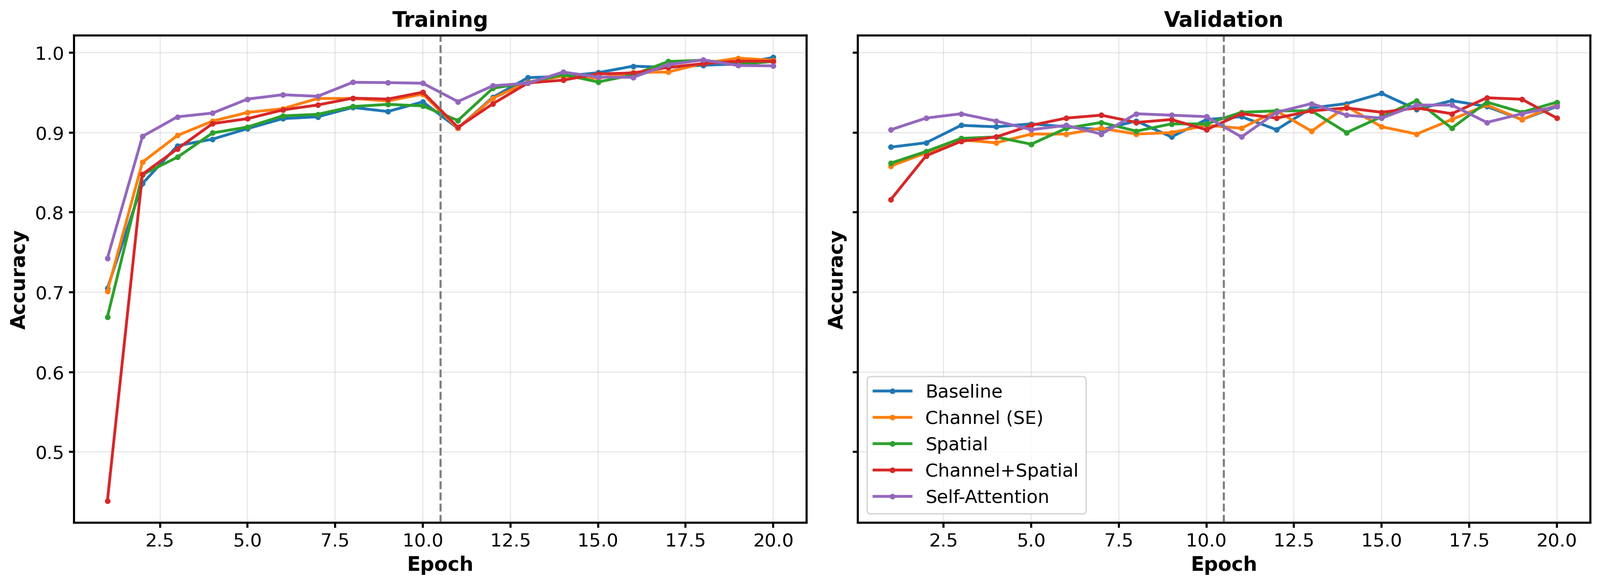
\includegraphics[width=\textwidth]{plots/02_accuracy_curves.png}
\caption{Training (left) and validation (right) accuracy against epoch. The dashed line marks the start of fine-tuning.}
\label{fig:acc}
\end{figure}
Self-attention starts fastest and Channel+Spatial slowest, but all models end near 99\% training and 92\% to 94\% validation accuracy. None is clearly better. Training accuracy dips at epoch 11 when conv5\_x is unfrozen and then climbs again, while validation accuracy stays at about 90\% to 94\% from epoch 3 onwards.

At the last epoch training accuracy is 5 to 7 points above validation accuracy for every model (6.15 points for the baseline, 7.13 for Channel+Spatial), so attention does not close this gap. After fine-tuning all validation curves move up and down by about 2 points, and no attention model is smoother than the baseline.

% ============================================================
\subsection*{25.2 Training and Validation Loss}
% ============================================================

\begin{figure}[!htbp]
\centering
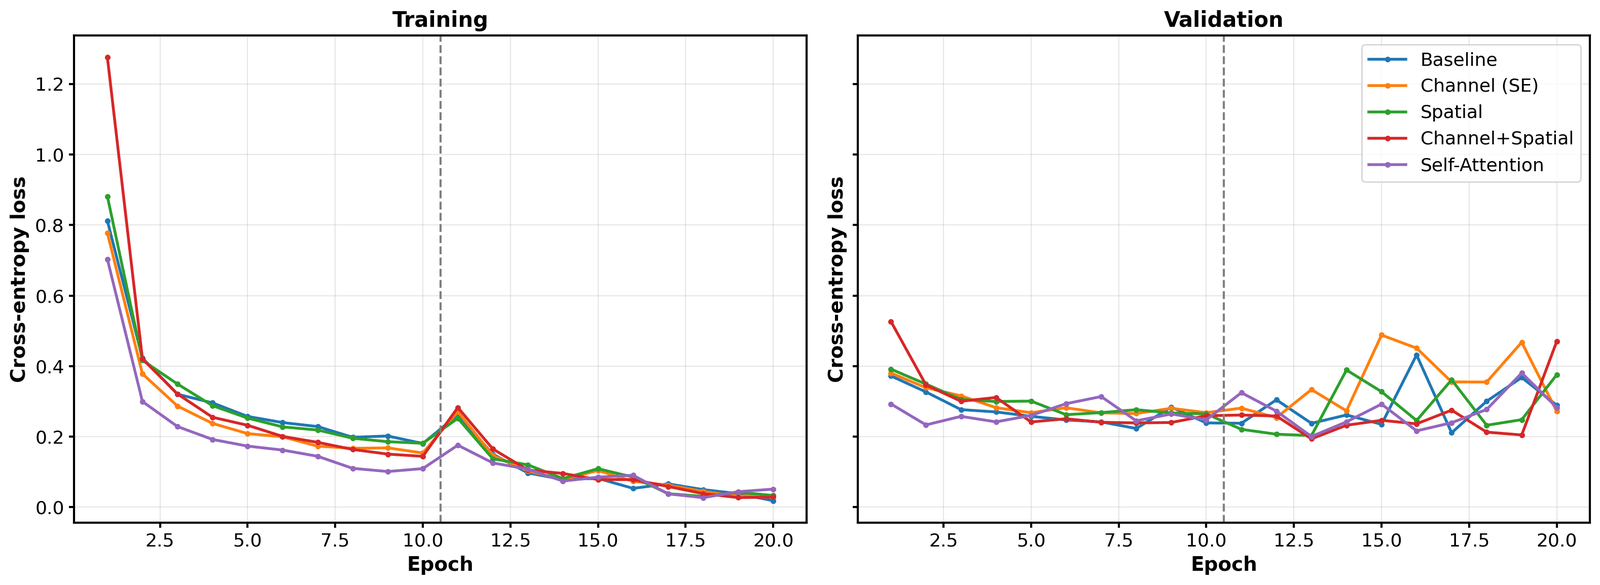
\includegraphics[width=\textwidth]{plots/03_loss_curves.png}
\caption{Training (left) and validation (right) loss against epoch. The dashed line marks the start of fine-tuning.}
\label{fig:loss}
\end{figure}
Validation loss stops improving after epochs 12 to 17 and then moves up and down while training loss keeps falling. So the models overfit, and last-epoch values are noisy. For example, Channel+Spatial jumps from about 0.20 at epoch 19 to 0.47 at epoch 20, which is why its last-epoch validation loss is the highest in the tables.

% ============================================================
\subsection*{25.3 Attention Mechanism versus Accuracy}
% ============================================================

\begin{figure}[!htbp]
\centering
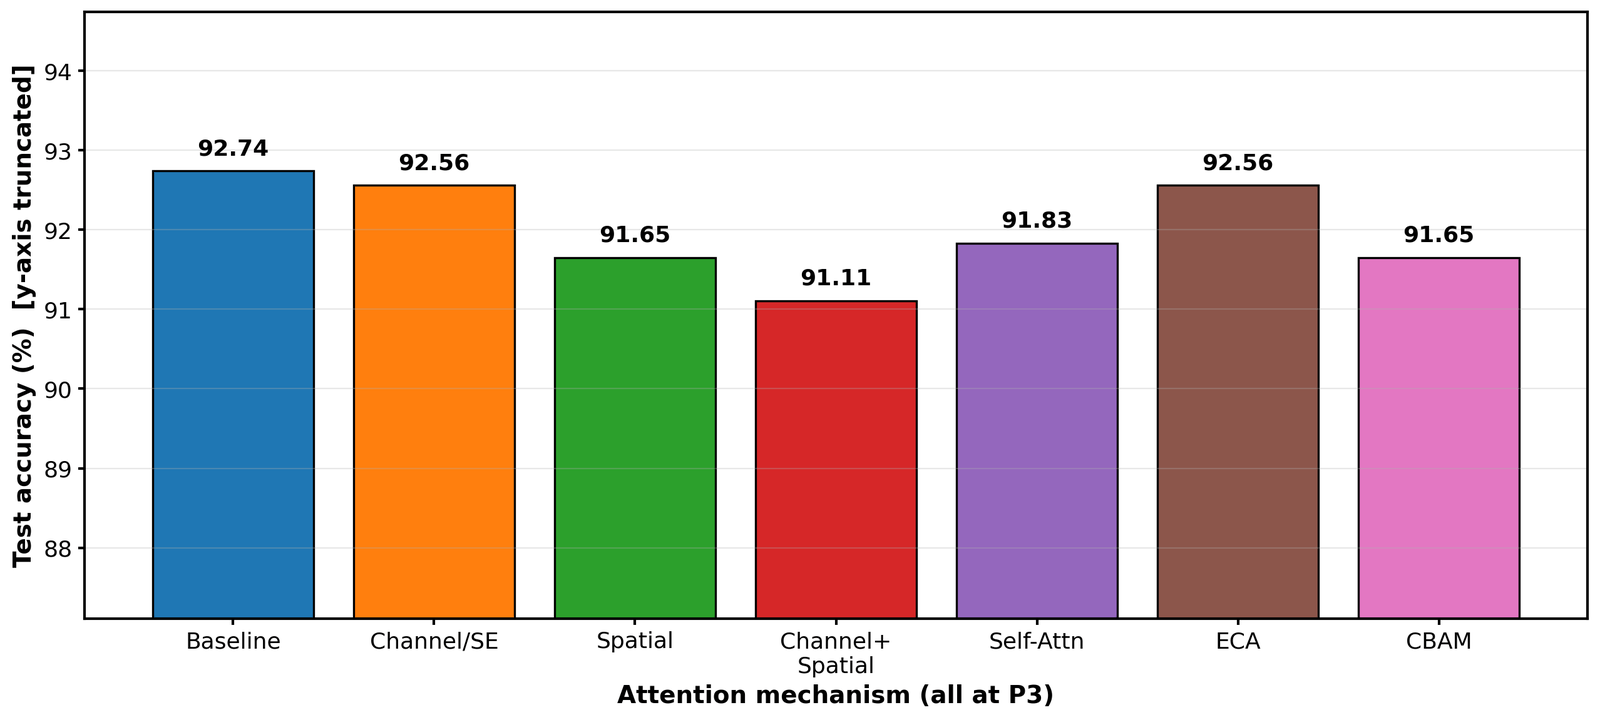
\includegraphics[width=0.8\textwidth]{plots/05_bar_accuracy.png}
\caption{Test accuracy of the attention mechanisms at $P_3$. The vertical axis does not start at zero.}
\label{fig:baracc}
\end{figure}
The baseline is the highest bar (92.74\%) and Channel+Spatial the lowest (91.11\%). The axis does not start at zero, so the 1.6 point gap (9 images) looks bigger than it is. The bars fall into two groups: SE and ECA sit just under the baseline at 92.56\%, and spatial, CBAM, self-attention and Channel+Spatial sit lower, between 91.11\% and 91.83\%.

% ============================================================
\subsection*{25.4 Attention Mechanism versus Macro F1}
% ============================================================

This comparison is useful when the class-wise performance is not uniform.

\begin{figure}[!htbp]
\centering
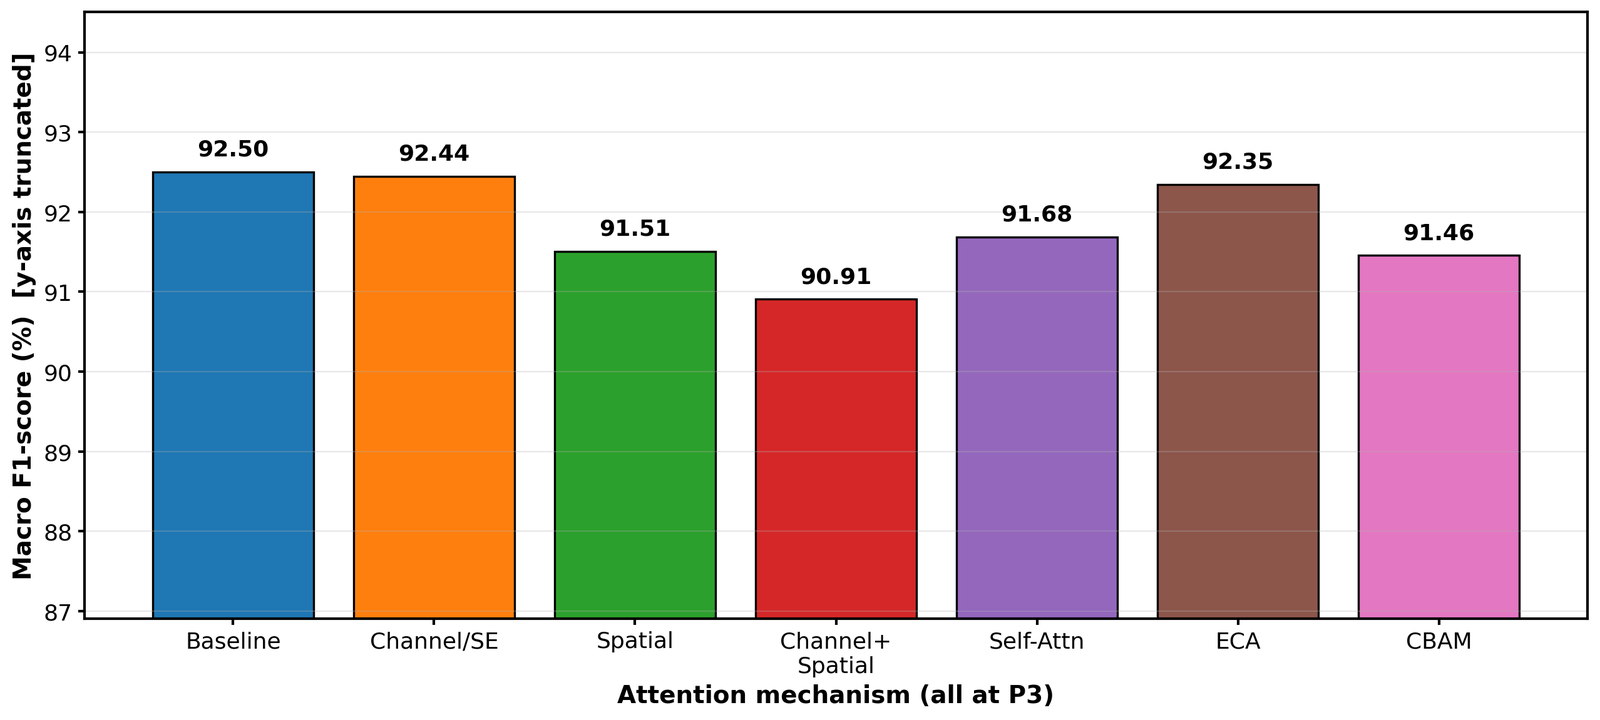
\includegraphics[width=0.8\textwidth]{plots/06_bar_macro_f1.png}
\caption{Macro F1-score of the attention mechanisms at $P_3$. The vertical axis does not start at zero.}
\label{fig:barf1}
\end{figure}
Macro F1 gives the same order as accuracy, from 92.50\% for the baseline to 90.91\% for Channel+Spatial. So the class-wise results do not change the ranking. The two channel-only mechanisms are again closest to the baseline, with SE at 92.44\% and ECA at 92.35\%.

% ============================================================
\subsection*{25.5 Accuracy versus Model Parameters}
% ============================================================

\begin{figure}[!htbp]
\centering
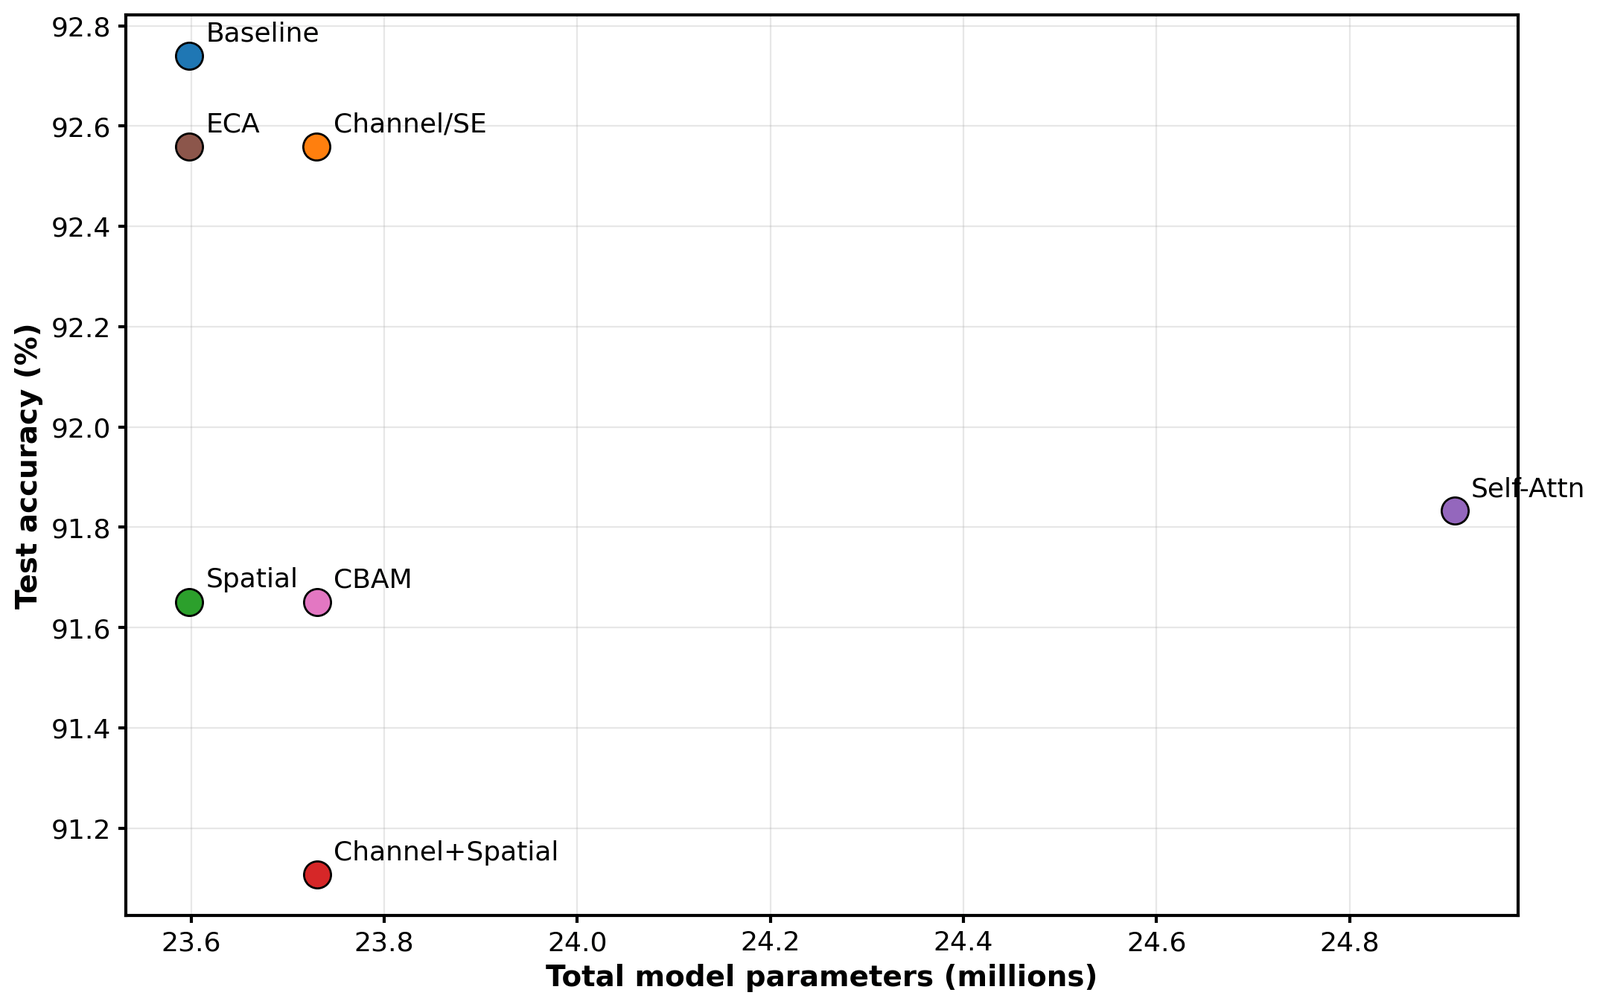
\includegraphics[width=0.72\textwidth]{plots/07_scatter_accuracy_vs_params.png}
\caption{Test accuracy against total parameters at $P_3$.}
\label{fig:scatter1}
\end{figure}
Only self-attention has clearly more parameters (24.91 million) and its accuracy is lower than the baseline. More parameters did not give higher accuracy. The other mechanisms all add less than 0.14 million parameters, and among them ECA, which adds almost nothing, ties for the best accuracy.

% ============================================================
\subsection*{25.6 Macro F1 versus Inference Time}
% ============================================================

\begin{figure}[!htbp]
\centering
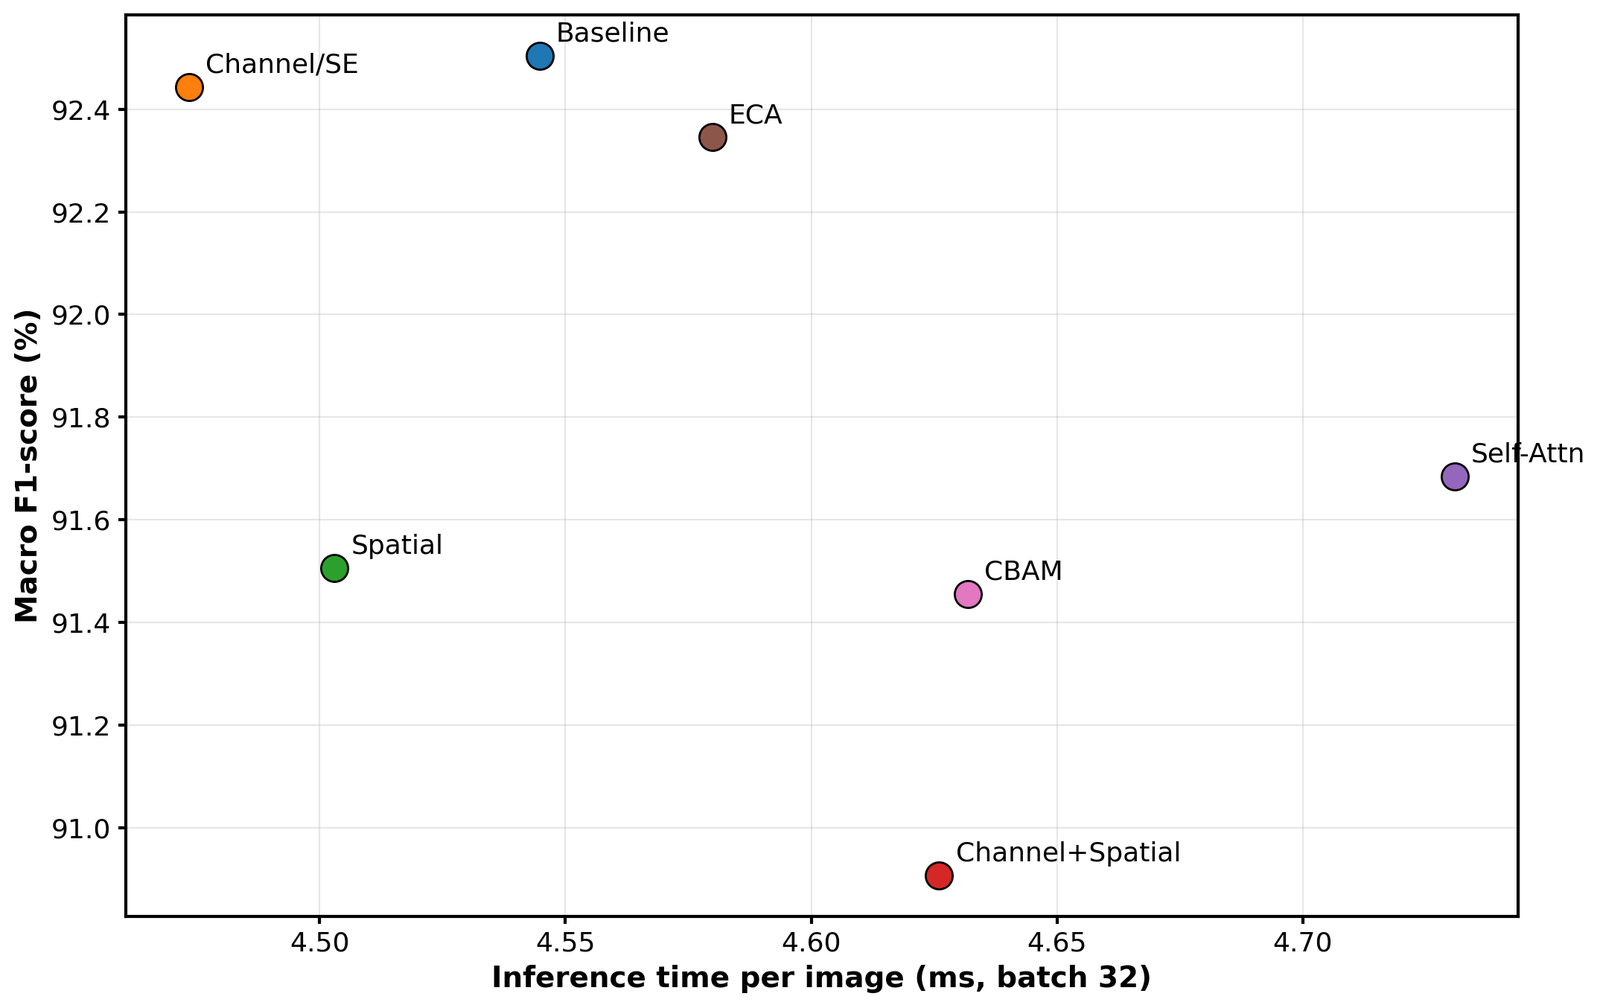
\includegraphics[width=0.72\textwidth]{plots/08_scatter_f1_vs_inference_time.png}
\caption{Macro F1-score against inference time per image at $P_3$.}
\label{fig:scatter2}
\end{figure}
The times lie between 4.47 and 4.73 ms per image, so the differences are small. Self-attention is the slowest and has a lower F1 than the baseline, so the extra time gave no gain. SE is the fastest model (4.47 ms) and also has the highest F1 among the attention models, so being slower did not mean being better.

% ============================================================
\section*{26. Confusion Matrix Analysis}
% ============================================================

\begin{figure}[!htbp]
\centering
\begin{subfigure}[t]{0.48\textwidth}
\centering
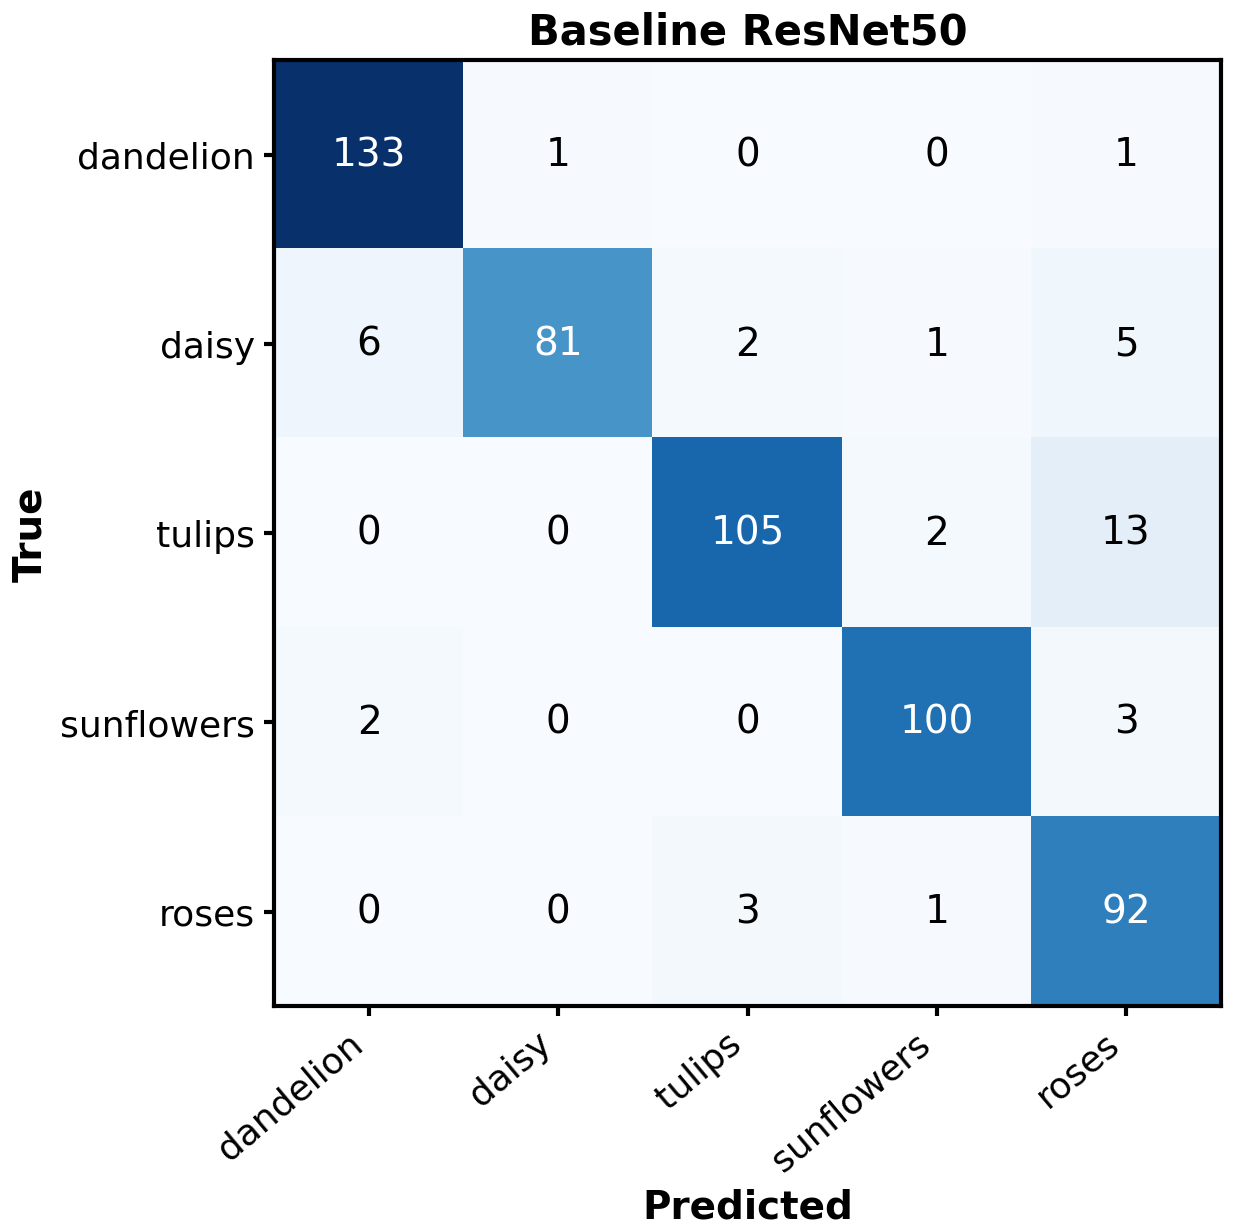
\includegraphics[width=\textwidth]{plots/04a_confusion_baseline.png}
\caption{Baseline ResNet50}
\label{fig:cmbase}
\end{subfigure}\hfill
\begin{subfigure}[t]{0.48\textwidth}
\centering
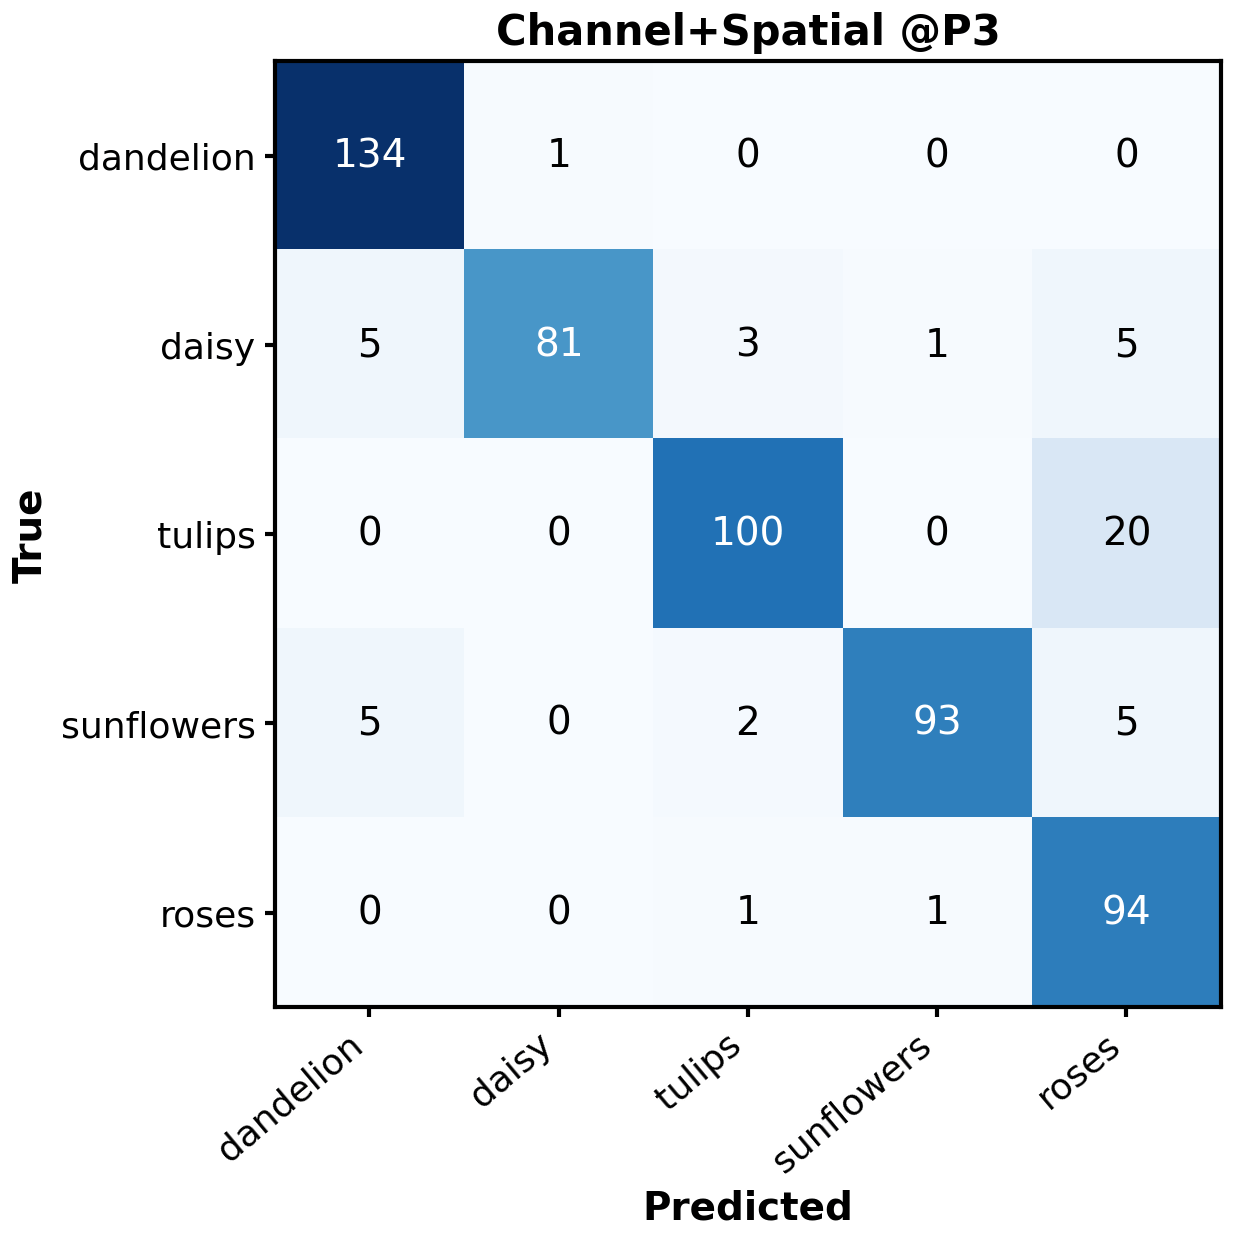
\includegraphics[width=\textwidth]{plots/04b_confusion_attention.png}
\caption{Channel+Spatial at $P_3$ (A3)}
\label{fig:cmatt}
\end{subfigure}
\medskip
\begin{subfigure}[t]{0.48\textwidth}
\centering
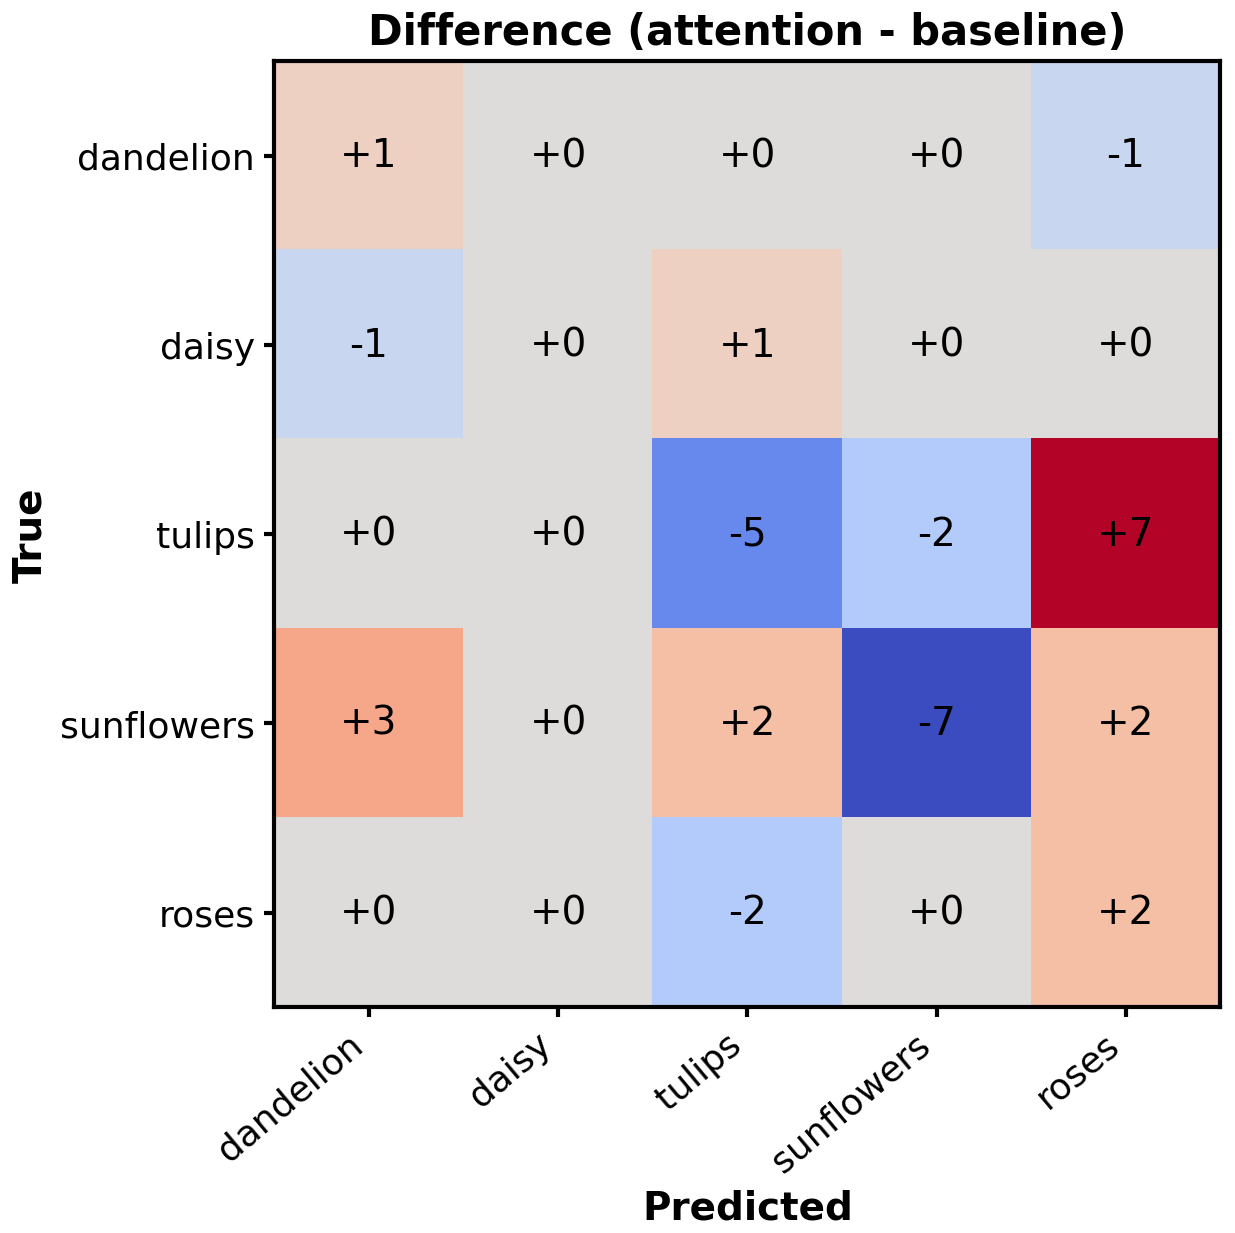
\includegraphics[width=\textwidth]{plots/04c_confusion_difference.png}
\caption{Difference (A3 minus baseline)}
\label{fig:cmdiff}
\end{subfigure}
\caption{Confusion matrices on the 551 test images (counts). Rows are the true classes and columns the predicted classes.}
\label{fig:cm}
\end{figure}
Tulips are most often predicted as roses (13 images in the baseline, 20 with A3). A3 loses 5 tulips and 7 sunflowers and gains 2 roses and 1 dandelion. Most of the lost sunflowers go to dandelion (3 images), probably because both are yellow. The daisy count on the diagonal does not change.

Dandelion and sunflowers are the best classified classes, with baseline F1 of 96.38\% and 95.69\%. A3 does not reduce any particular confusion. The biggest one, tulips predicted as roses, actually goes up, and the 9 lost images come mostly from tulips and sunflowers, so the change is not spread evenly across classes.

\begin{table}[H]
\centering
\caption{Class-wise F1-score (\%) for all sixteen runs.}
\begin{tabular}{|l|c|c|c|c|c|}
\hline
\textbf{Run} & \textbf{dandelion} & \textbf{daisy} & \textbf{tulips} & \textbf{sunflowers} & \textbf{roses}\\
\hline
A0 & 96.38 & 91.53 & 91.30 & 95.69 & 87.62 \\
\hline
A1 & 95.65 & 93.41 & 89.08 & 97.12 & 86.96 \\
\hline
A2 & 94.93 & 94.51 & 87.70 & 95.73 & 84.66 \\
\hline
A3 & 96.06 & 91.53 & 88.50 & 93.00 & 85.45 \\
\hline
A4 & 96.24 & 92.97 & 87.65 & 95.69 & 85.86 \\
\hline
A5 & 93.24 & 93.41 & 90.00 & 96.19 & 87.83 \\
\hline
B1 & 93.82 & 89.13 & 89.33 & 94.06 & 87.23 \\
\hline
B2 & 94.96 & 92.31 & 88.98 & 97.61 & 83.80 \\
\hline
B4 & 95.02 & 95.08 & 87.50 & 94.93 & 86.49 \\
\hline
M34 & 96.32 & 92.31 & 89.08 & 96.71 & 87.31 \\
\hline
M234 & 94.29 & 91.71 & 89.06 & 97.58 & 83.15 \\
\hline
O\_SC & 97.01 & 94.57 & 91.29 & 97.17 & 89.34 \\
\hline
K3 & 95.34 & 92.13 & 86.53 & 90.82 & 88.24 \\
\hline
K5 & 96.70 & 94.62 & 90.13 & 96.19 & 88.00 \\
\hline
ECA & 97.04 & 92.90 & 90.43 & 96.19 & 85.17 \\
\hline
CBAM & 95.94 & 92.39 & 88.89 & 94.34 & 85.71 \\
\hline
\end{tabular}
\end{table}

Daisy has a higher F1 than the baseline in 13 of the 15 attention runs, while tulips are lower in all 15. So attention helps daisy but hurts tulips, and the overall accuracy does not improve. Tulips and roses are the two weakest classes in 15 of the 16 runs, which fits the colour overlap seen in the sample images.

% ============================================================
\section*{27. Qualitative Analysis of Attention}
% ============================================================

Quantitative classification performance does not directly explain where the
network obtains evidence for its prediction.

\begin{figure}[!htbp]
\centering
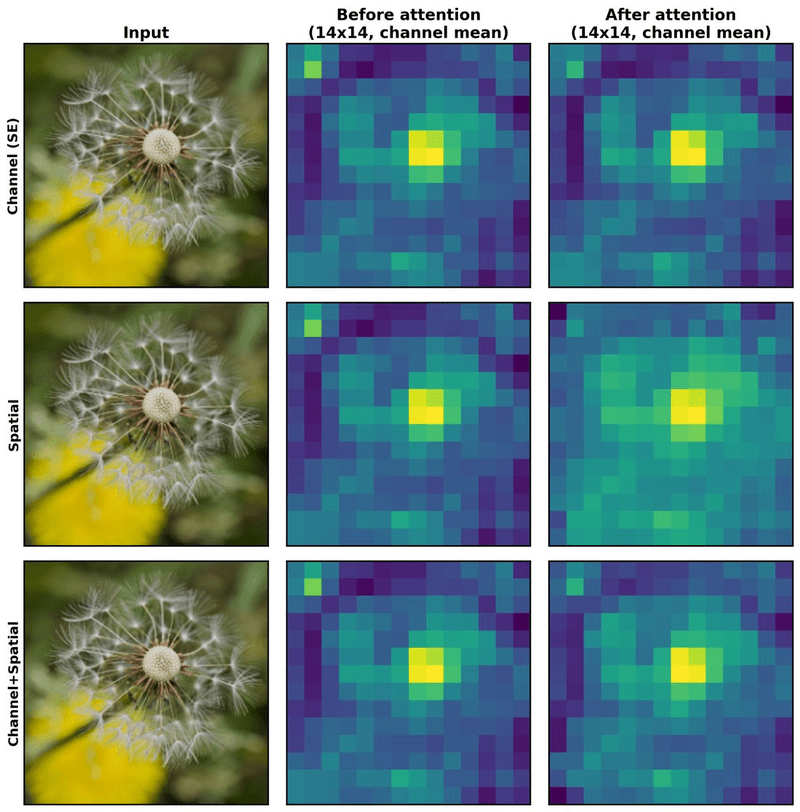
\includegraphics[width=0.6\textwidth]{plots/10_feature_maps_before_after.png}
\caption{Channel-averaged feature map at $P_3$ before and after attention (rows: channel, spatial, Channel+Spatial; columns: input, before, after).}
\label{fig:featmap}
\end{figure}
The channel mean map looks almost the same before and after attention. The centre of the seed head stays the brightest in all three rows. The spatial and Channel+Spatial rows dim the bright cell in the top-left corner a little, which matches the low border values of the spatial map. Otherwise the attention only rescales the map.

% ============================================================
\section*{28. Grad-CAM Visualization}
% ============================================================

Gradient-weighted Class Activation Mapping (Grad-CAM) provides a
class-specific visualization of the regions contributing to a prediction.

Let

\[
A^k
\]

represent feature map $k$ from a selected convolutional layer.

For class score $y^c$, the importance coefficient is:

\[
\alpha_k^c
=
\frac{1}{HW}
\sum_i
\sum_j
\frac{\partial y^c}
{\partial A_{ij}^k}.
\]

The Grad-CAM map is:

\[
L_{\mathrm{Grad-CAM}}^c
=
\operatorname{ReLU}
\left(
\sum_k
\alpha_k^c A^k
\right).
\]

\begin{figure}[!htbp]
\centering
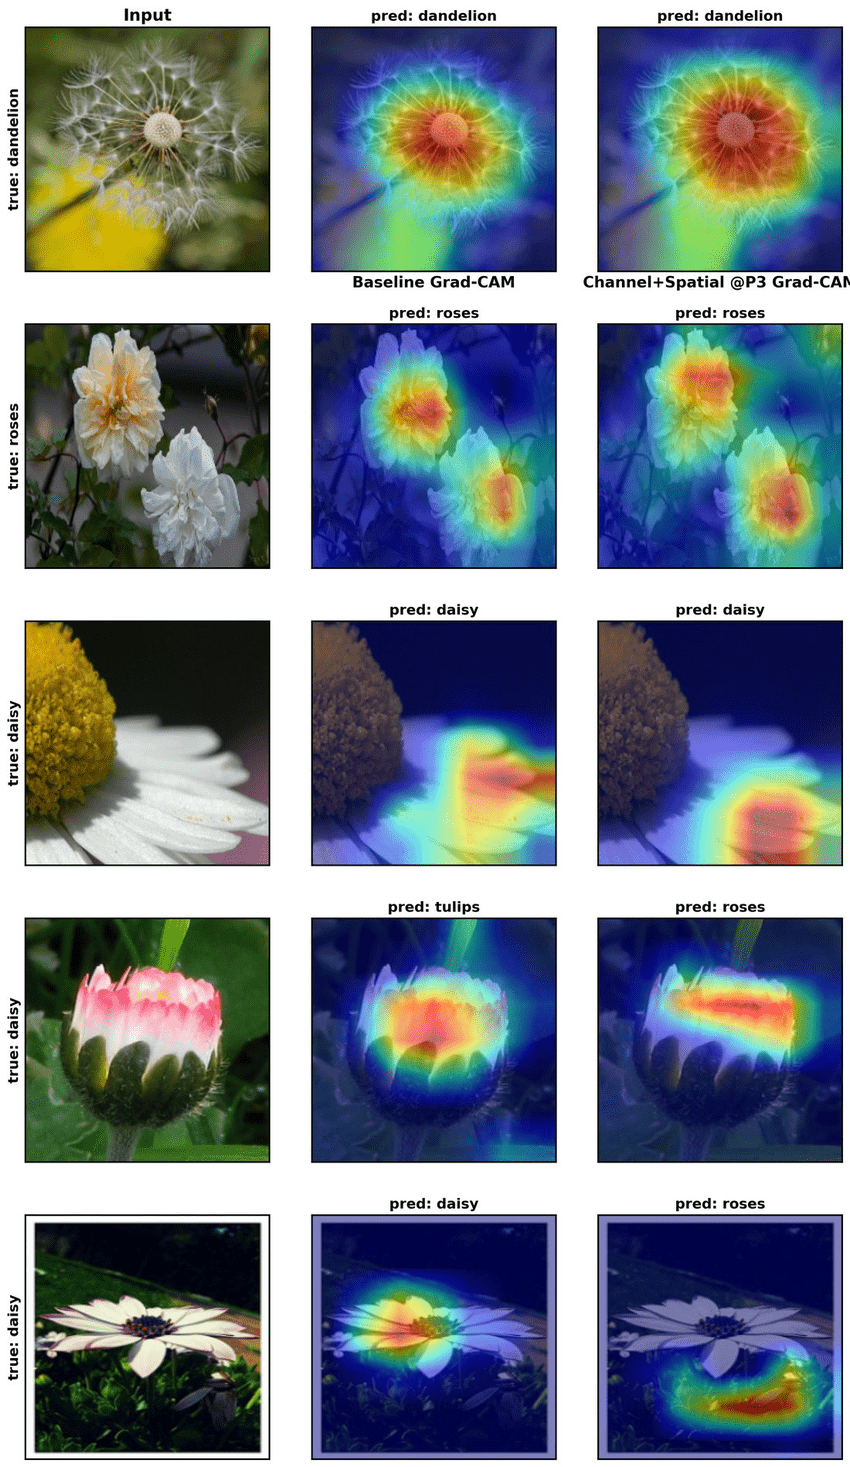
\includegraphics[width=0.62\textwidth]{plots/16_gradcam_baseline_vs_attention.png}
\caption{Input, baseline Grad-CAM and Channel+Spatial Grad-CAM for three correct and two incorrect test images (predicted class above each map).}
\label{fig:gc}
\end{figure}
On the three correct images both models look at the same flower regions. For the last daisy image the attention model looks at the ground below the flower and predicts roses. On the fourth daisy both models are wrong (tulips and roses), and the attention map becomes a narrow band on the petal tips.

% ============================================================
\subsection*{28.1 Grad-CAM Interpretation}
% ============================================================

\begin{itemize}
\item \textbf{Focus on the flower:} not stronger. On the correct images both models look at the same regions.
\item \textbf{Background suppression:} not visible. The baseline already has low activation on the background.
\item \textbf{Petals:} yes for the daisy images, in both models.
\item \textbf{Central structure:} both models activate the dandelion seed head, but neither activates the yellow centre of the daisy close-up.
\item \textbf{Edges:} not visible, as the maps are smooth blobs at $7\times7$ size.
\item \textbf{Whole flower:} in the roses image both models cover both flowers.
\item \textbf{Leaves:} only in the last daisy image, where the attention model's map lies on the ground and plants below the flower. The baseline puts almost no activation on leaves.
\item \textbf{Background objects:} in the dandelion image both models give weak activation on the blurred yellow flower in the bottom-left corner, and attention does not remove it.
\item \textbf{Incorrect prediction:} yes. The attention maps change for both incorrect images.
\end{itemize}

% ============================================================
\section*{29. Internal Attention Maps}
% ============================================================

An important objective of this experiment is to distinguish between:

\[
\boxed{\text{Internal Attention}}
\]

and

\[
\boxed{\text{Post-hoc Explanation}}
\]

because they are not the same.

An attention module directly computes weights during the forward pass.

Grad-CAM, in contrast, is generated after prediction using gradients.

% ============================================================
\subsection*{29.1 Channel-Attention Visualization}
% ============================================================

For channel attention:

\[
M_c(F)
=
[m_1,m_2,\ldots,m_C].
\]

\begin{figure}[!htbp]
\centering
\begin{subfigure}[t]{0.48\textwidth}
\centering
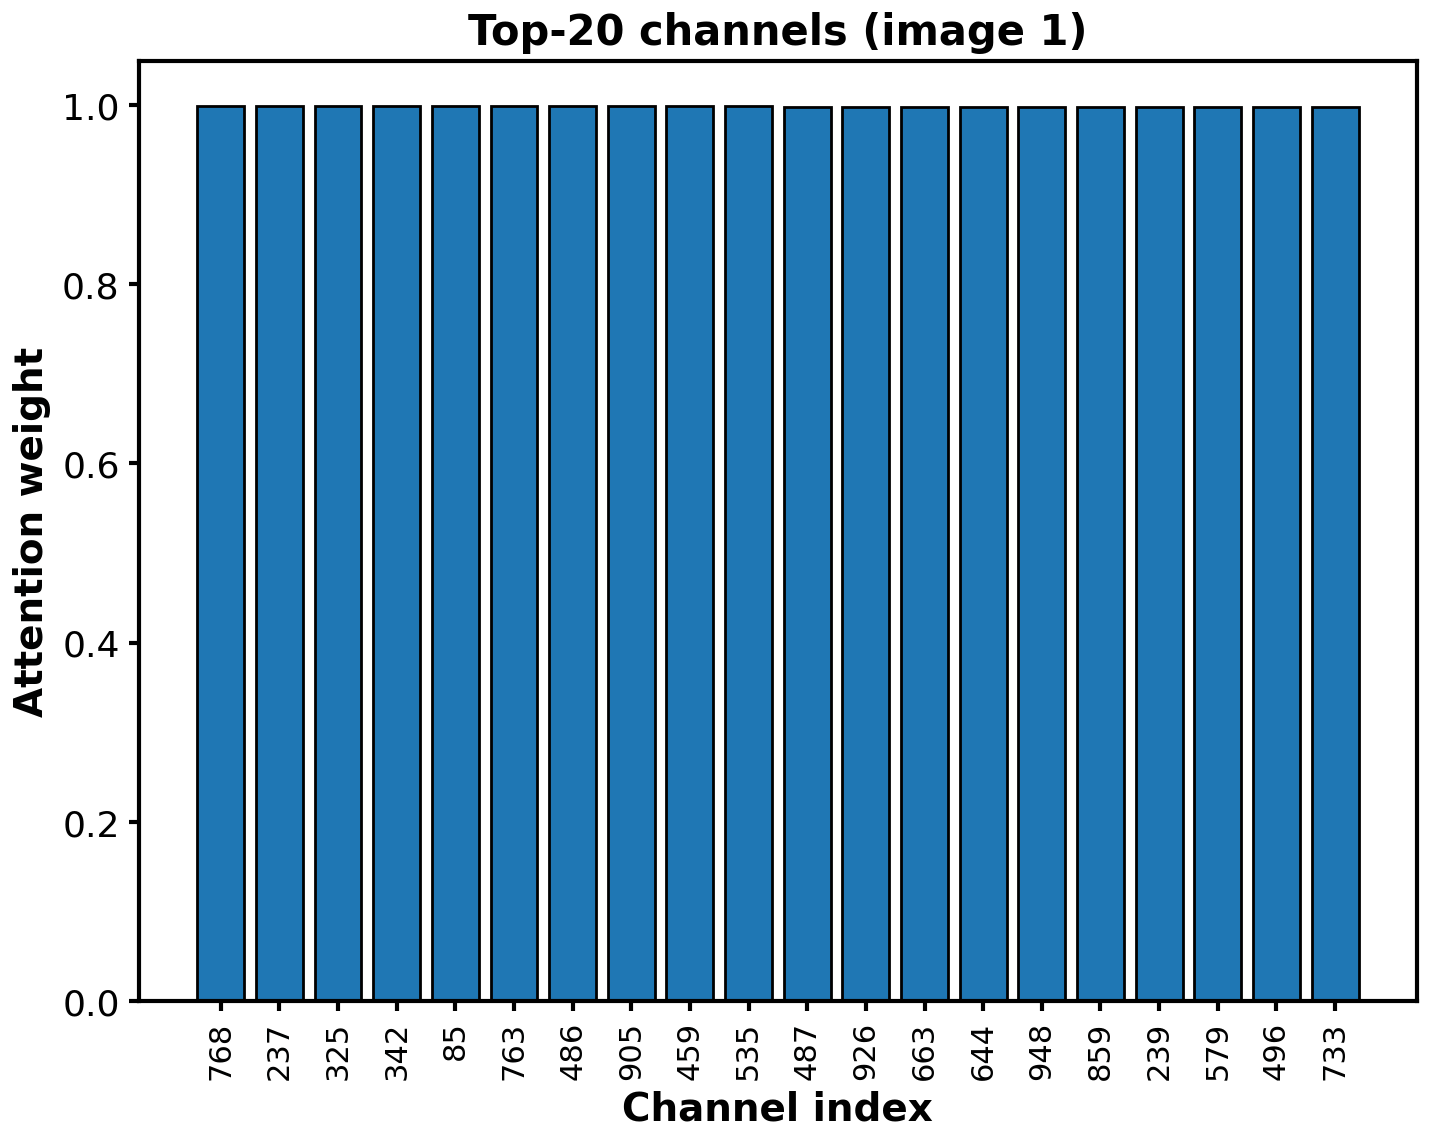
\includegraphics[width=\textwidth]{plots/11a_channel_top20.png}
\caption{Top-20 channels of image 1}
\label{fig:chw1}
\end{subfigure}\hfill
\begin{subfigure}[t]{0.48\textwidth}
\centering
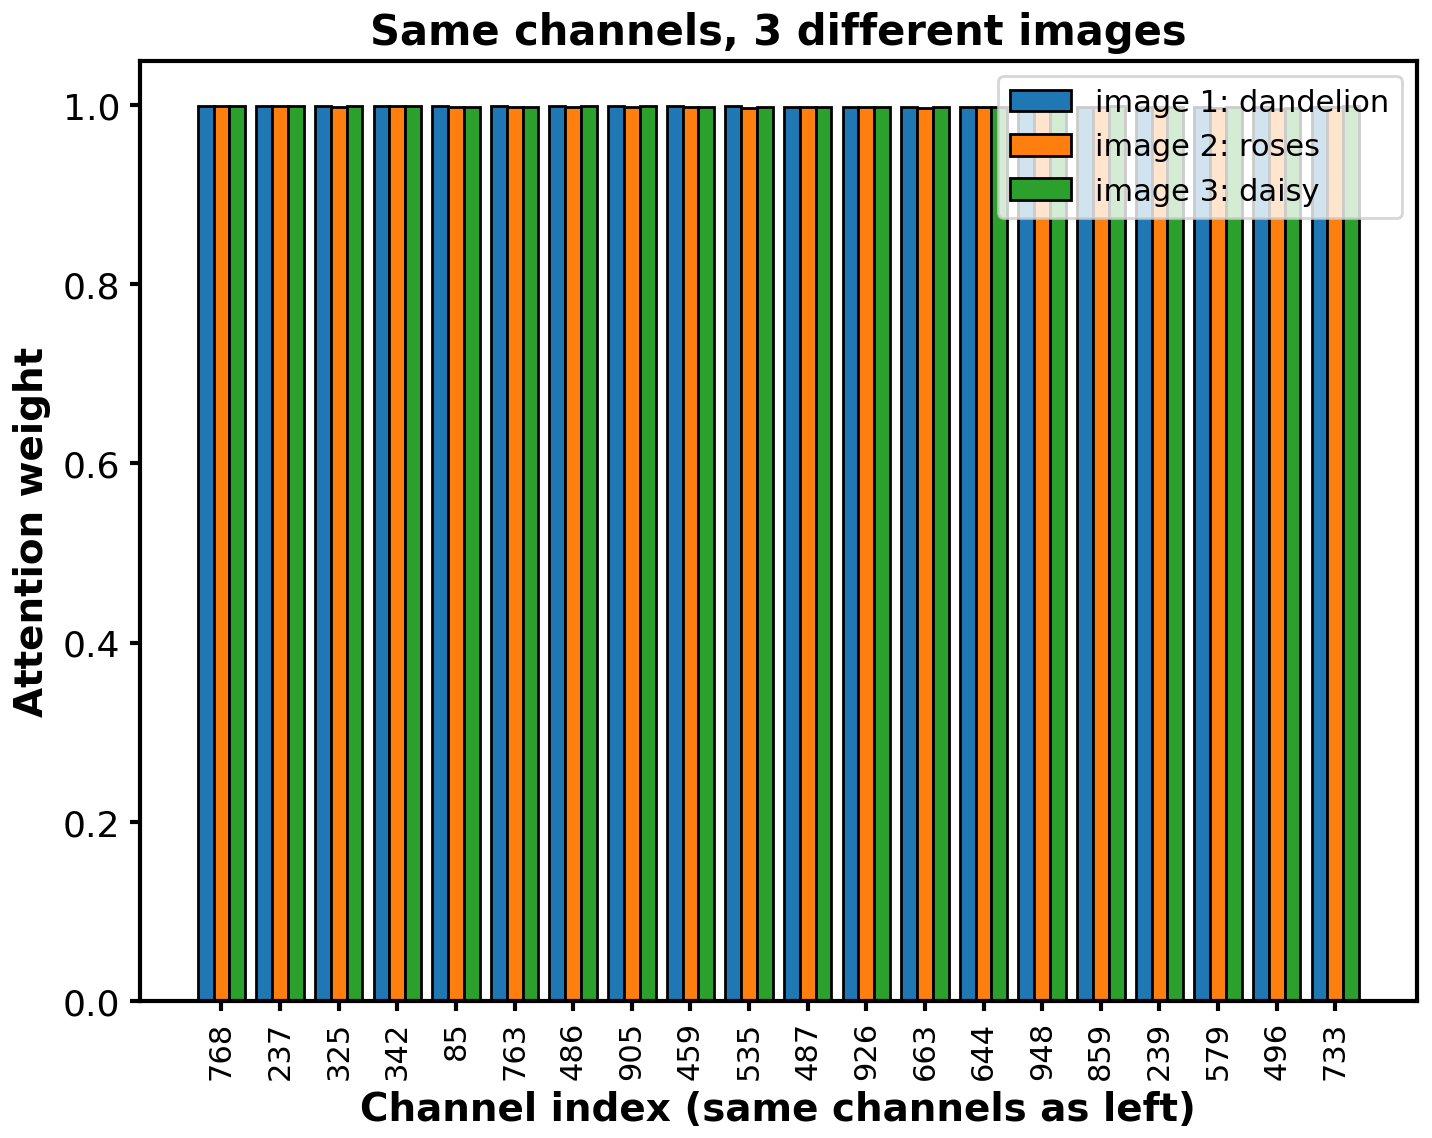
\includegraphics[width=\textwidth]{plots/11b_channel_three_images.png}
\caption{Same channels, three images}
\label{fig:chw2}
\end{subfigure}
\medskip
\begin{subfigure}[t]{0.48\textwidth}
\centering
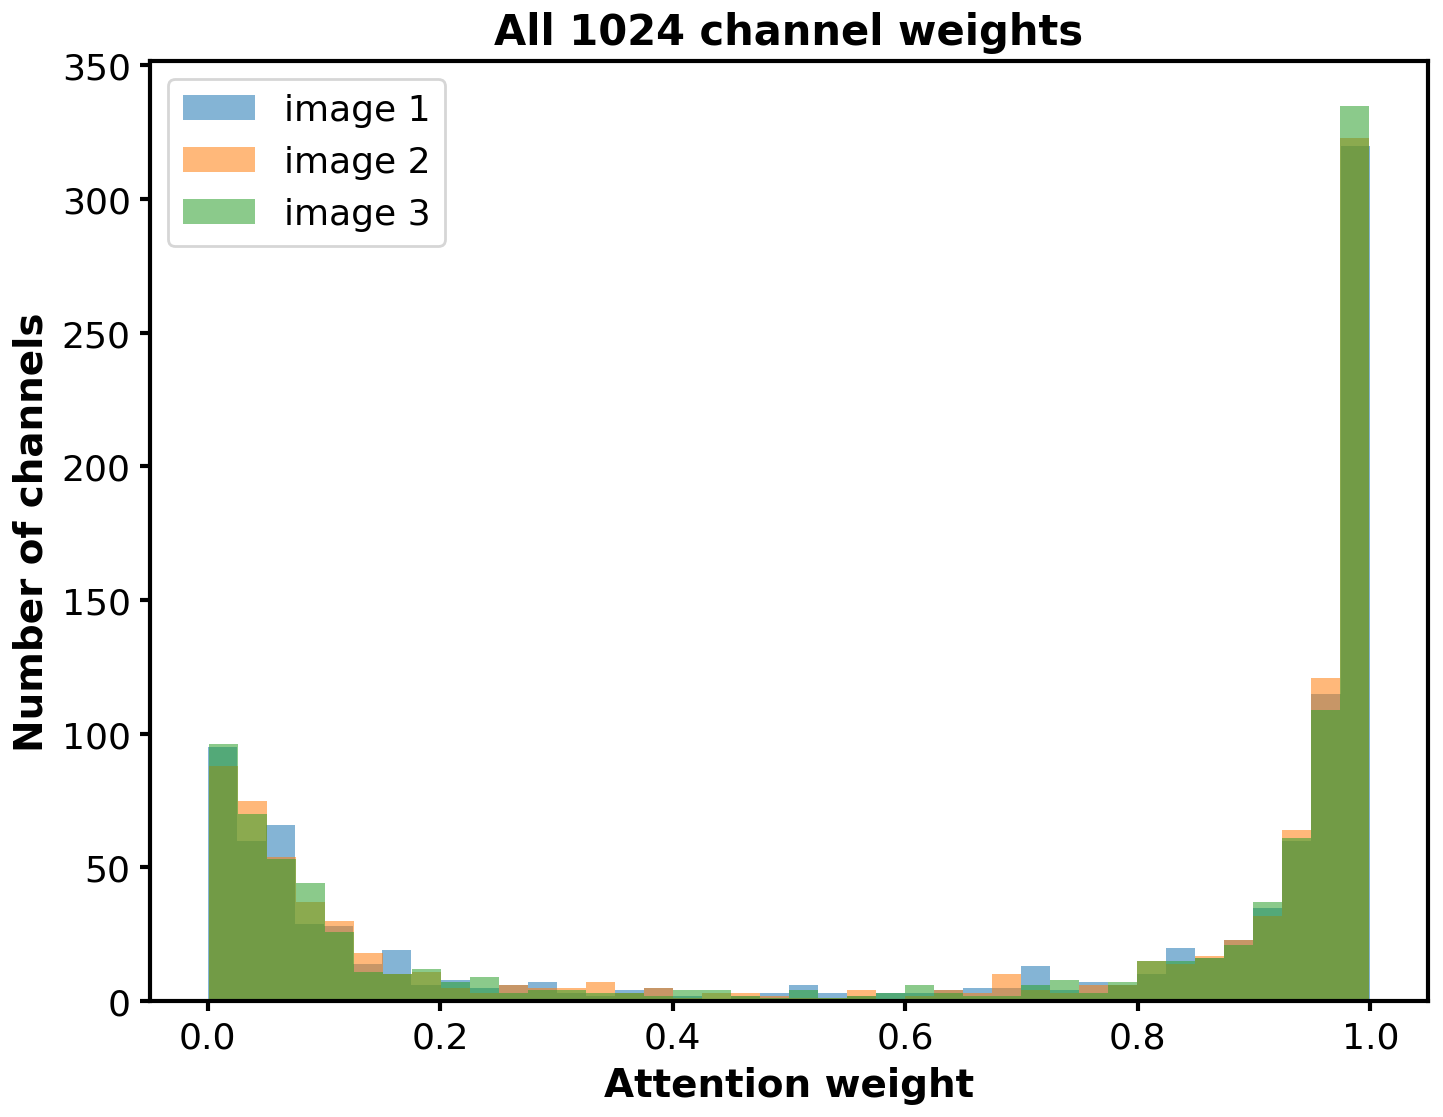
\includegraphics[width=\textwidth]{plots/11c_channel_histogram.png}
\caption{All 1024 channel weights}
\label{fig:chw3}
\end{subfigure}
\caption{Channel-attention weights of the channel (SE) model at $P_3$. Images 1 to 3 are the dandelion, roses and daisy test images.}
\label{fig:chw}
\end{figure}
About a third of the channels are near 0 and the rest near 1, and the weights are almost the same for every image. So channel attention works like a fixed mask. Very few channels fall between 0.2 and 0.8 in the histogram, so the gate is close to an on/off switch learned during training rather than something that adapts to each flower.

% ============================================================
\subsection*{29.2 Spatial-Attention Visualization}
% ============================================================

For spatial attention:

\[
M_s(F)
\in
\mathbb{R}^{H\times W}.
\]

\begin{figure}[!htbp]
\centering
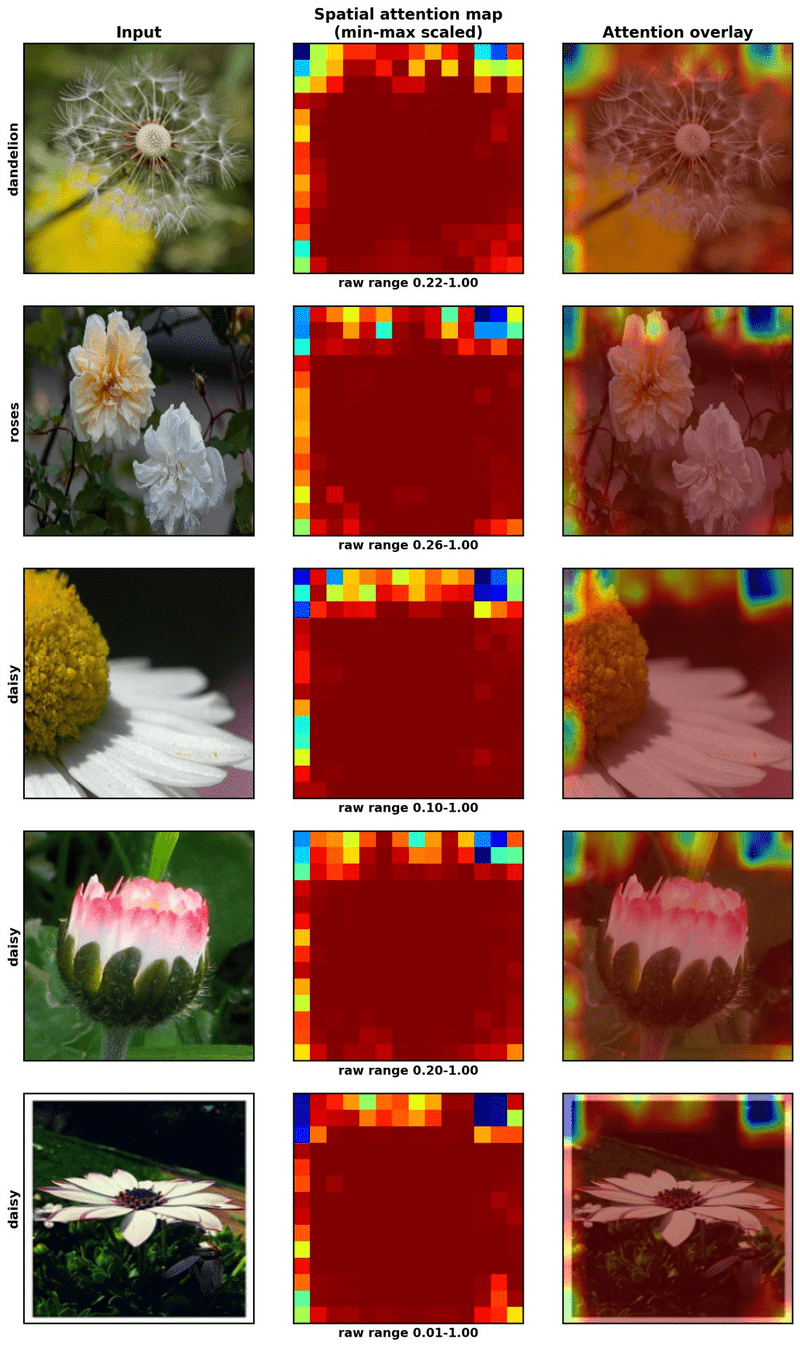
\includegraphics[width=0.55\textwidth]{plots/12_spatial_attention_overlay.png}
\caption{Spatial attention (A2, $P_3$) for the five test images: input, map (scaled to its own minimum and maximum) and overlay. The raw range is written under each map.}
\label{fig:spatial}
\end{figure}
The map is flat inside (mean 0.94) and changes only at the image border, so it does not highlight the flower. The low values sit mostly along the top and left edges, and the raw minimum ranges from 0.01 to 0.26 between images. This looks like an effect of zero padding in the $7\times7$ convolution rather than anything learned about the flower.

% ============================================================
\subsection*{29.3 Self-Attention Visualization}
% ============================================================

\begin{figure}[!htbp]
\centering
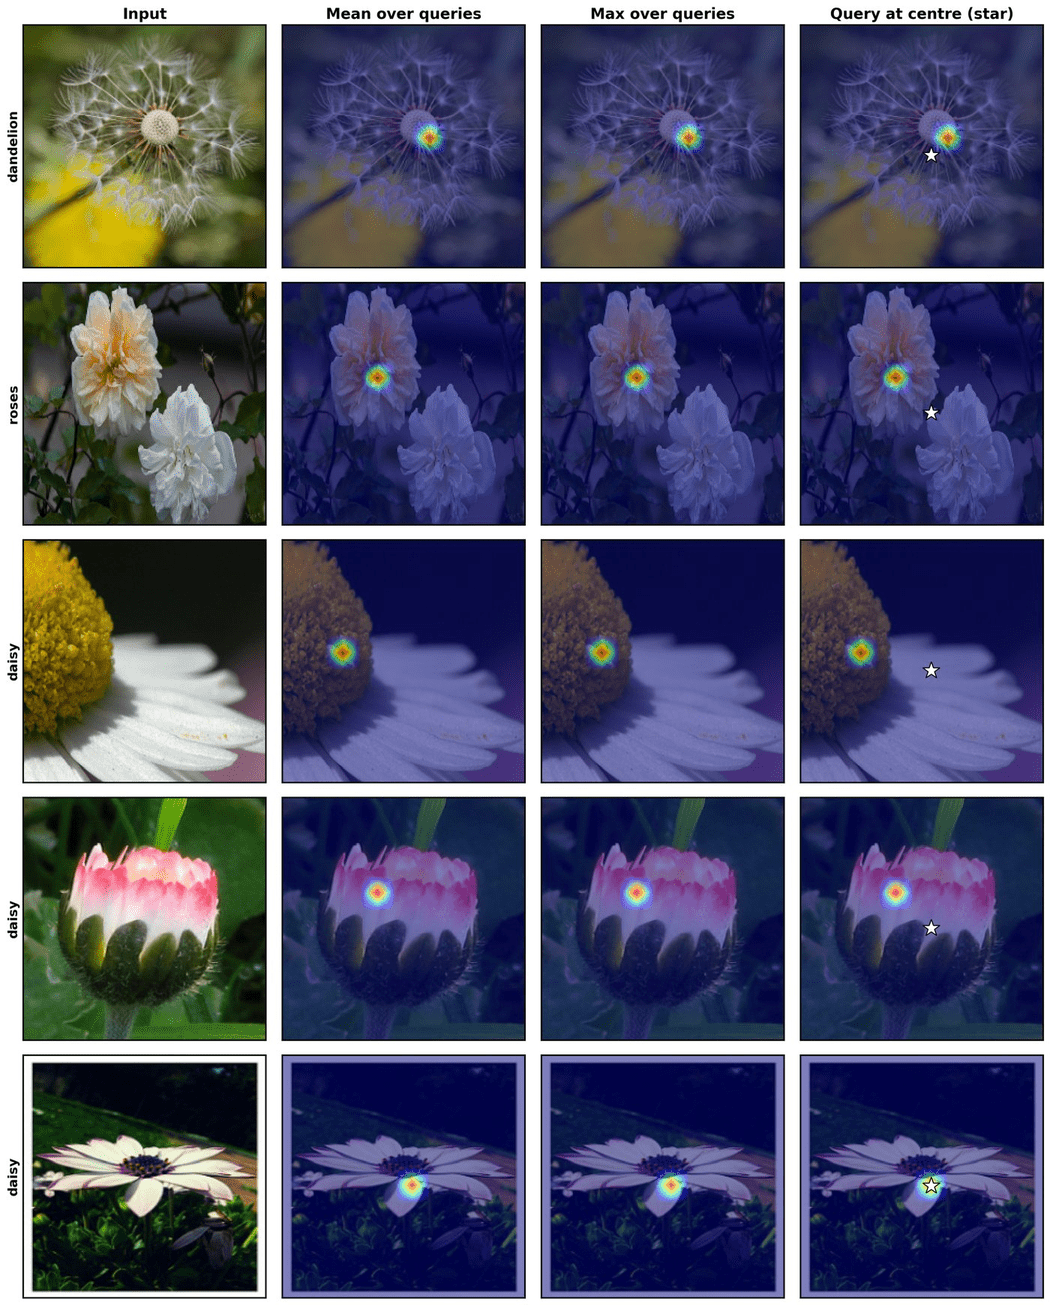
\includegraphics[width=0.78\textwidth]{plots/14_self_attention_response.png}
\caption{Self-attention response of A4 at $P_3$: input, mean over queries, maximum over queries and the query at the centre (star).}
\label{fig:selfatt}
\end{figure}
The response is one spot on the flower, the same for every query, and the scale $\gamma$ is only $-0.02$. So this module barely changes the features. The mean, maximum and centre-query maps are almost identical, which means every location attends to the same single position. That spot is not always on the most useful part either, for example in the roses image it lies only on the left flower.

So distant regions do not really interact in this module. A query on the petals and a query on the background both take their features from the same spot, instead of linking related parts of the flower to each other.

% ============================================================
\section*{30. Attention Position Visualization}
% ============================================================

The objective is to visually study how attention changes as feature
representations become deeper.

Possible observations may include:

\begin{itemize}

\item $P_2$ responding strongly to edges, colors, textures, and fine
structures;

\item $P_3$ responding to flower parts and intermediate object structures;

\item $P_4$ responding to larger semantic flower regions.

\end{itemize}

\begin{figure}[!htbp]
\centering
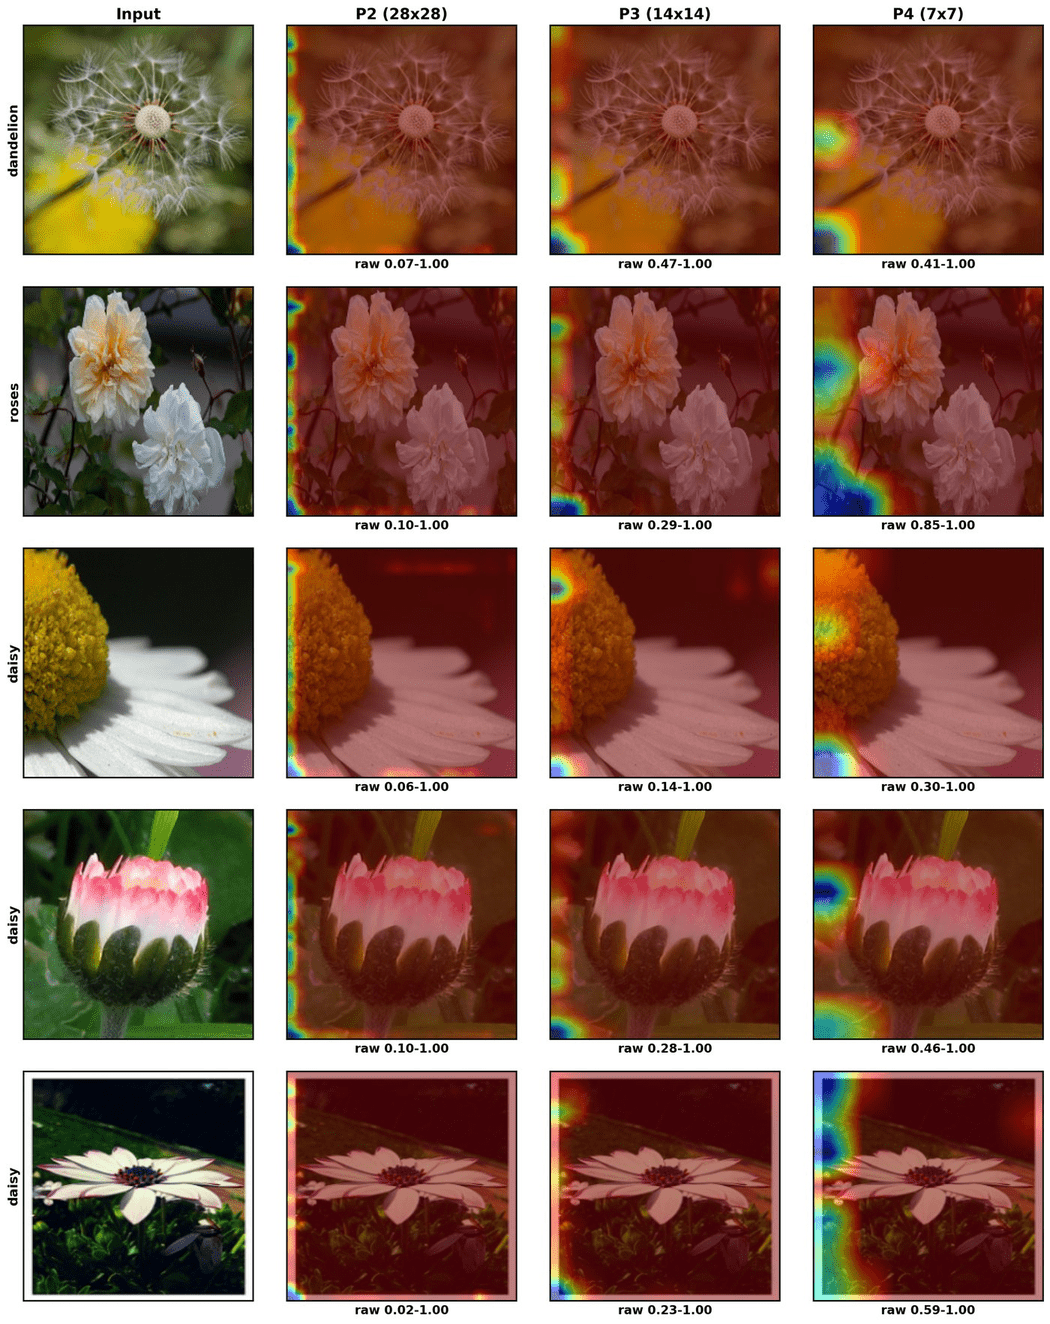
\includegraphics[width=0.78\textwidth]{plots/15_spatial_attention_P2_P3_P4.png}
\caption{Spatial attention maps at $P_2$, $P_3$ and $P_4$ for the five test images (models B2, A3 and B4). Raw minimum values are written under each map.}
\label{fig:pos}
\end{figure}
\begin{table}[H]
\centering
\caption{Statistics of the spatial attention maps over 100 test images.}
\begin{tabular}{|l|c|c|c|}
\hline
\textbf{Model (position)} & \textbf{Mean value} & \textbf{Minimum} & \textbf{Locations above 0.5}\\
\hline
B2 ($P_2$) & 0.978 & 0.002 & 98.4\%\\
\hline
A3 ($P_3$) & 0.983 & 0.093 & 99.3\%\\
\hline
B4 ($P_4$) & 0.973 & 0.008 & 97.9\%\\
\hline
\end{tabular}
\end{table}

The maps at $P_2$, $P_3$ and $P_4$ look alike, with a flat interior and low values only at the border. So no change from edges to flower parts is seen with depth. The table agrees: at all three positions the mean is about 0.97 to 0.98 and over 97\% of locations are above 0.5, so almost everything passes through. Only the border blocks get bigger.

% ============================================================
\section*{31. Qualitative Comparison Across Attention Mechanisms}
% ============================================================

\begin{figure}[!htbp]
\centering
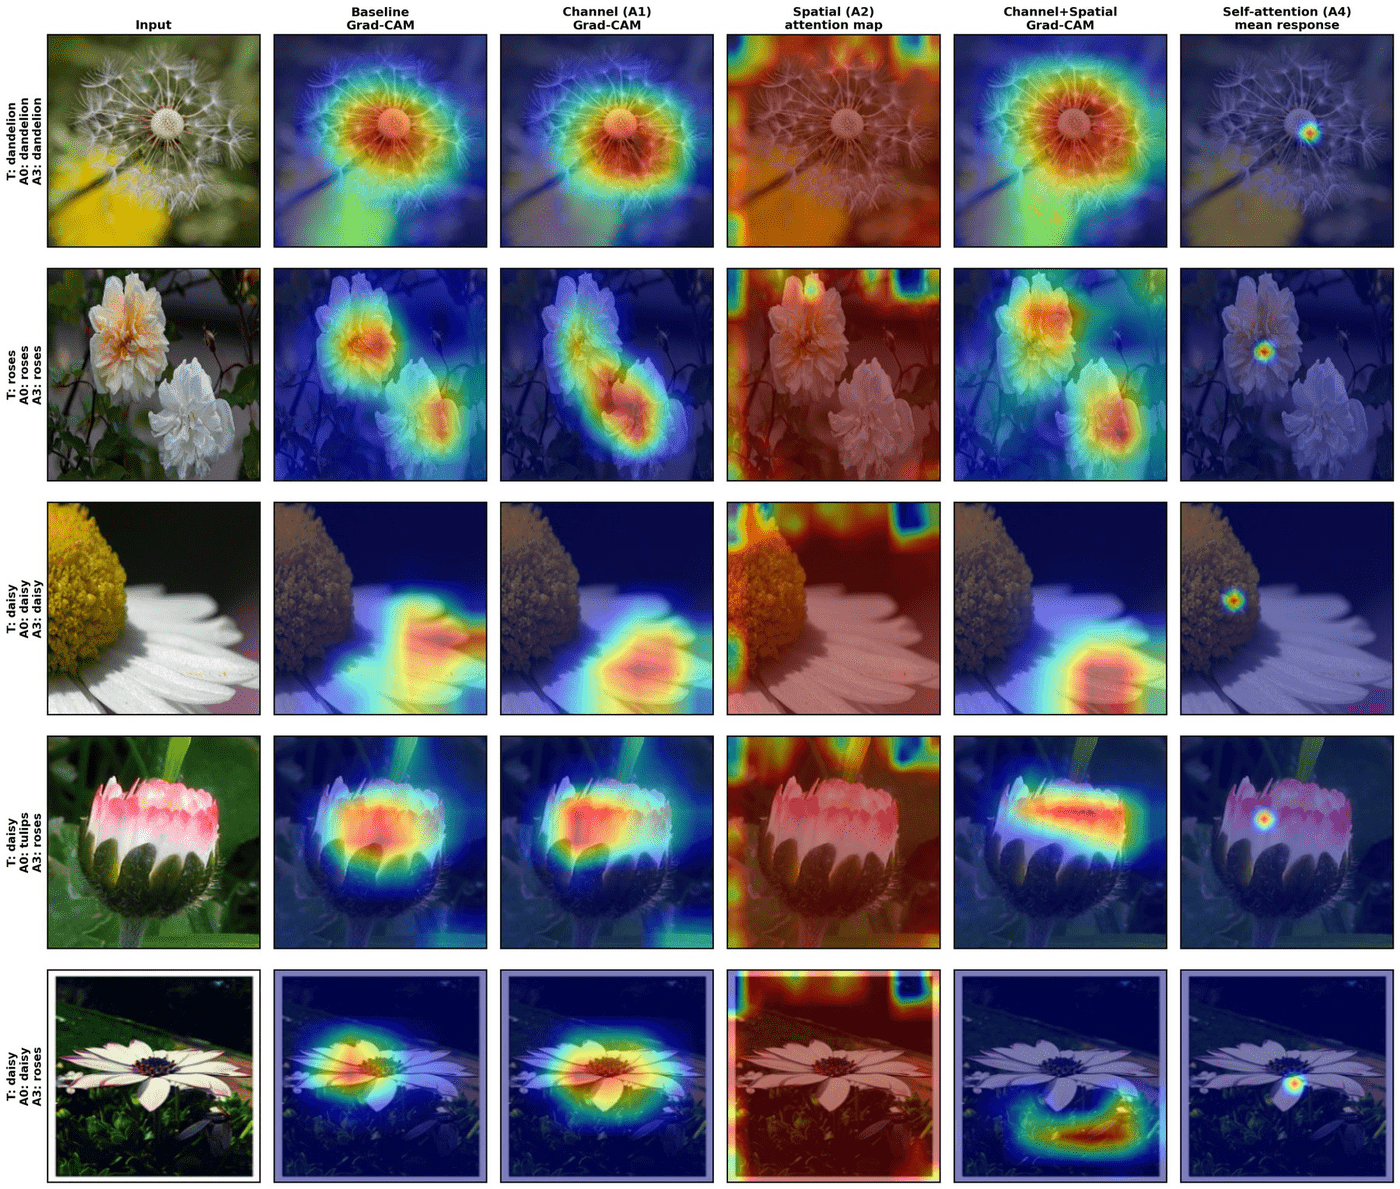
\includegraphics[width=\textwidth]{plots/17_qualitative_grid.png}
\caption{Three correct and two incorrect test images. Columns: input (T = true class, A0 = baseline prediction, A3 = Channel+Spatial prediction), baseline Grad-CAM, channel (A1) Grad-CAM, spatial (A2) map, Channel+Spatial (A3) Grad-CAM, self-attention (A4) response.}
\label{fig:grid}
\end{figure}
The maps look similar for the models on the correct images and differ on the two wrong ones. The spatial map is flat and the self-attention map is one spot. On the correct images even the A1 Grad-CAM is close to the baseline, except for roses where it joins both flowers. Both models miss image 4 and only A3 misses image 5.

% ============================================================
\subsection*{31.1 Qualitative Criteria}
% ============================================================

\begin{itemize}
\item \textbf{Foreground and background:} the Grad-CAM maps lie on the flower in all images except the last one for A3, and no background suppression is visible.
\item \textbf{Petals and centre:} the daisy maps lie on the petals, and the yellow centre of the close-up gets no activation.
\item \textbf{Compactness:} in the daisy close-up the A3 map is a compact block, and in the roses image the SE map is one region joining both flowers.
\item \textbf{Activation coverage:} the baseline and A1 maps cover most of the flower in the dandelion and daisy images, while the A3 map on the fourth image covers only a thin band of the petals.
\item \textbf{Incorrectly attended regions:} only the last image, where the A3 map lies on the ground below the flower.
\item \textbf{Correct against incorrect:} on the three correct images every Grad-CAM lies on the flower, while on the two wrong ones the A3 map shrinks to a band or moves off the flower.
\item \textbf{Consistency and depth:} the spatial maps show the same border pattern in every image and at every position, and the self-attention response is always one spot.
\end{itemize}

% ============================================================
\section*{32. Required Visualizations}
% ============================================================

\begin{enumerate}

\item Sample input images from all five classes;

\item Training and validation accuracy curves;

\item Training and validation loss curves;

\item Confusion matrix;

\item Feature map before attention;

\item Channel-attention weights;

\item Spatial-attention heatmap;

\item Spatial-attention overlay;

\item Self-attention response for the self-attention experiment;

\item Feature map after attention;

\item Baseline Grad-CAM;

\item Grad-CAM for at least one attention-based model;

\item Attention maps at $P_2$, $P_3$, and $P_4$; and

\item At least one graphical comparison of the performances of different
attention mechanisms.

\end{enumerate}

\medskip
\textbf{Where each required visualization is shown}

\begin{table}[H]
\centering
\caption{Required visualizations and the figures that contain them.}
\begin{tabular}{|c|l|c|}
\hline
\textbf{No.} & \textbf{Required visualization} & \textbf{Figure}\\
\hline
1 & Sample input images from all five classes & \ref{fig:samples}\\
\hline
2 & Training and validation accuracy curves & \ref{fig:acc}\\
\hline
3 & Training and validation loss curves & \ref{fig:loss}\\
\hline
4 & Confusion matrix & \ref{fig:cm}\\
\hline
5 & Feature map before attention & \ref{fig:featmap}\\
\hline
6 & Channel-attention weights & \ref{fig:chw}\\
\hline
7 & Spatial-attention heatmap & \ref{fig:spatial}\\
\hline
8 & Spatial-attention overlay & \ref{fig:spatial}\\
\hline
9 & Self-attention response & \ref{fig:selfatt}\\
\hline
10 & Feature map after attention & \ref{fig:featmap}\\
\hline
11 & Baseline Grad-CAM & \ref{fig:gc}\\
\hline
12 & Grad-CAM of an attention-based model & \ref{fig:gc}, \ref{fig:grid}\\
\hline
13 & Attention maps at $P_2$, $P_3$ and $P_4$ & \ref{fig:pos}\\
\hline
14 & Comparison of attention mechanisms & \ref{fig:baracc}, \ref{fig:barf1}, \ref{fig:abl}\\
\hline
\end{tabular}
\end{table}

% ============================================================
\section*{33. Recommended Visualization Layout}
% ============================================================

\begin{figure}[!htbp]
\centering
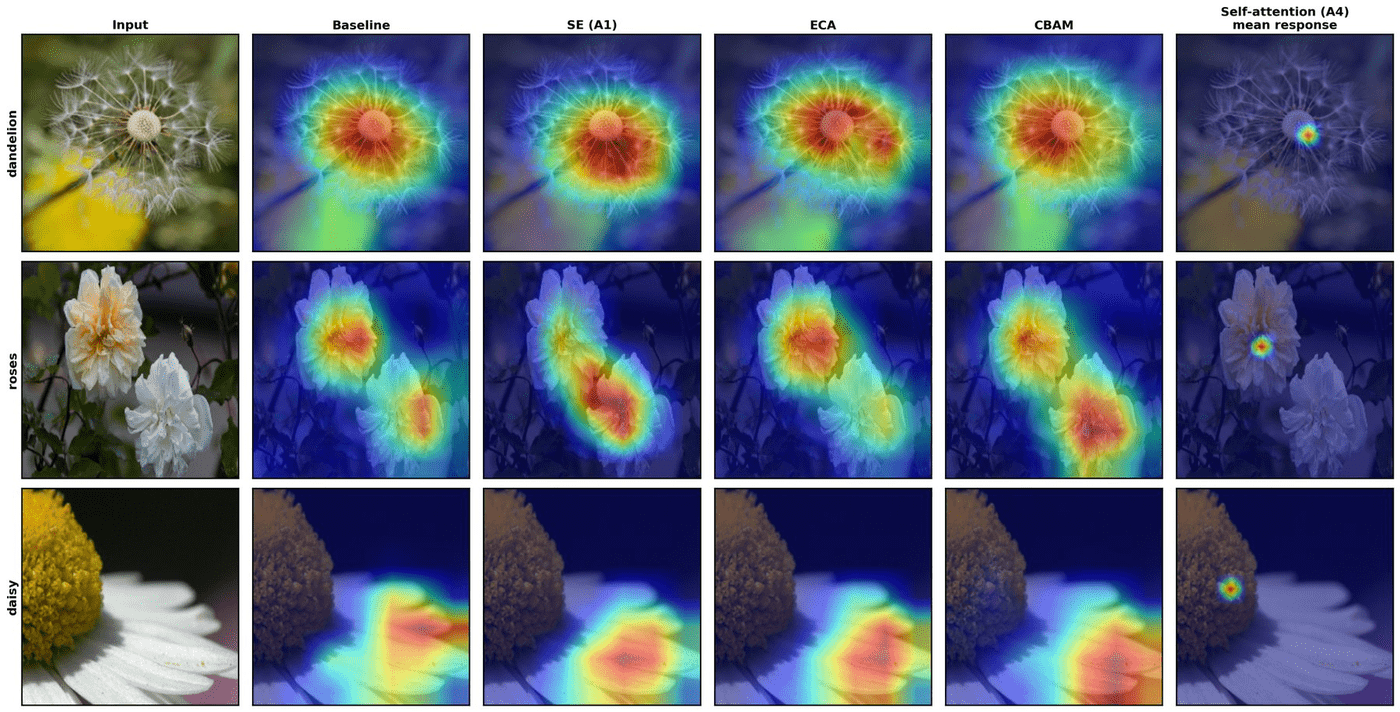
\includegraphics[width=\textwidth]{plots/18_gradcam_extended_SE_ECA_CBAM_SA.png}
\caption{Three correct images. Columns: input, baseline, SE (A1), ECA, CBAM and self-attention (A4) response.}
\label{fig:ext}
\end{figure}
SE, ECA and CBAM cover the same flower regions as the baseline with small shifts, and none of them activates the background. ECA looks the most like the baseline in all three images. In the roses image CBAM puts its peak on the right flower and SE stretches one region over both, while self-attention again gives one small spot.

% ============================================================
\section*{34. Required Experimental Analysis}
% ============================================================

\subsection*{34.1 Quantitative Analysis}

\[
\boxed{
\text{Accuracy}
+
\text{Precision}
+
\text{Recall}
+
\text{Macro F1}
}
\]

\begin{figure}[!htbp]
\centering
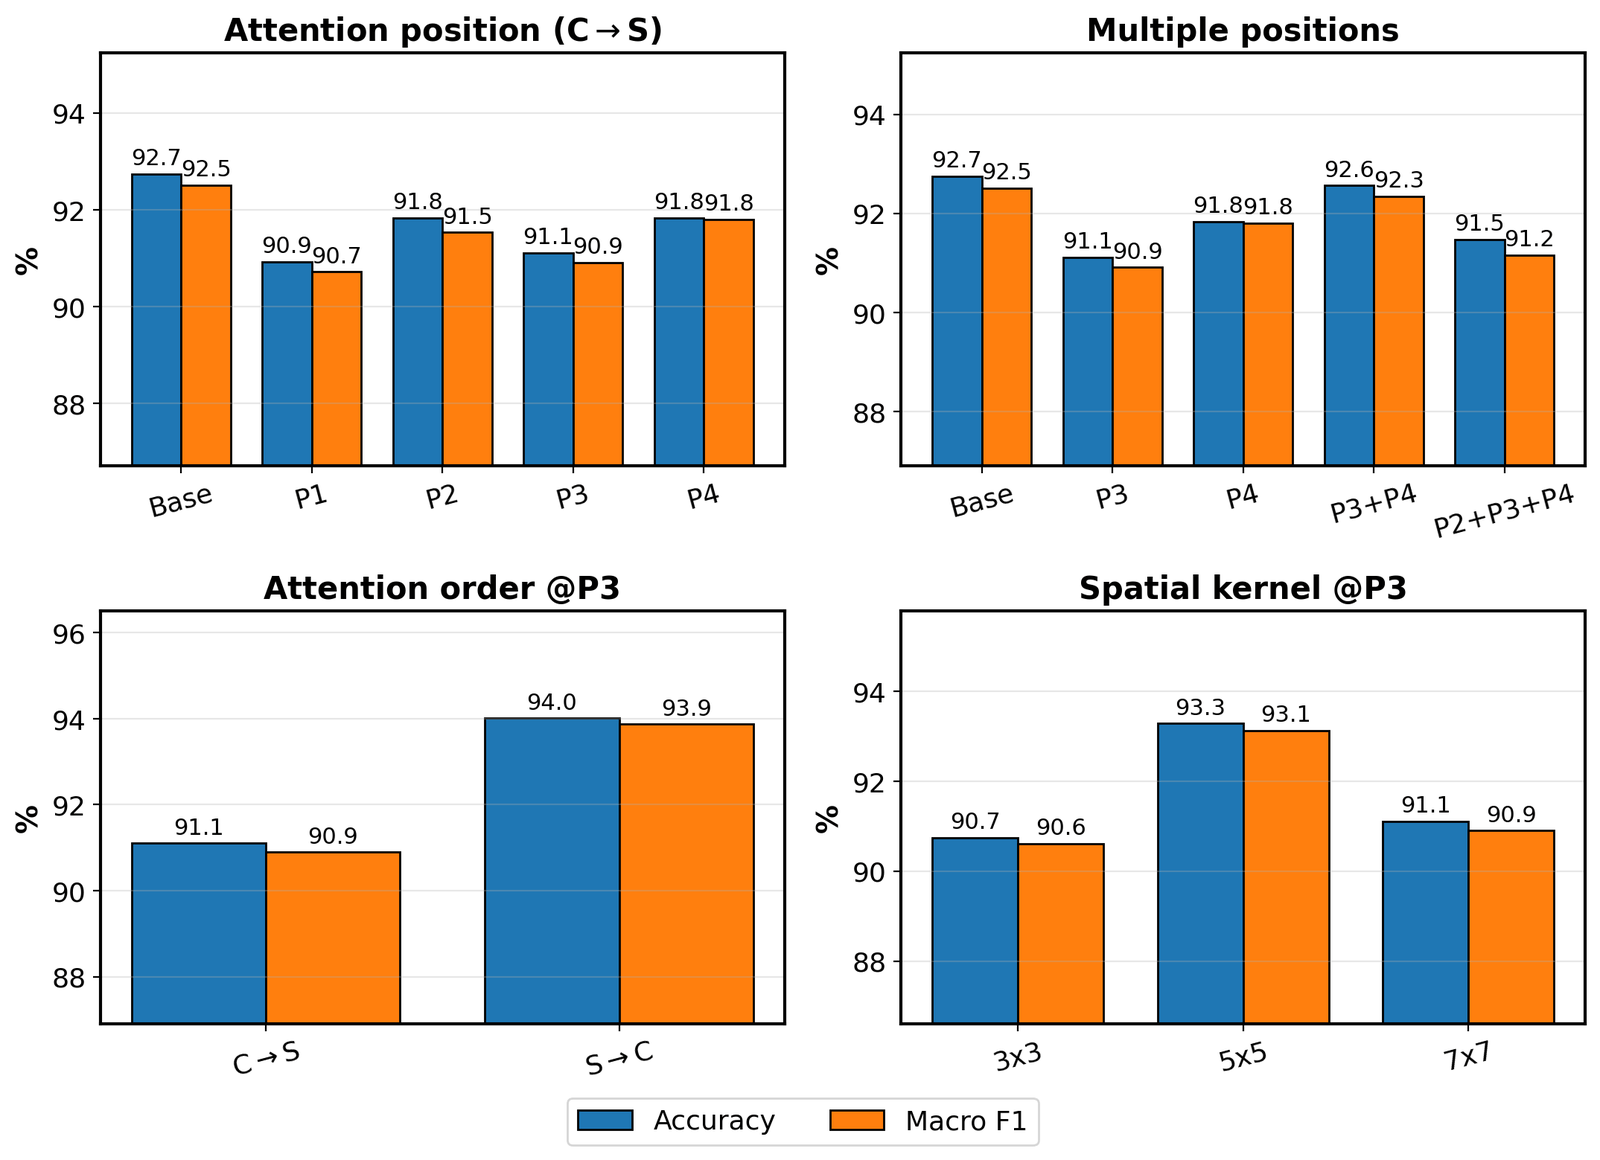
\includegraphics[width=0.85\textwidth]{plots/09_ablation_summary.png}
\caption{Accuracy and macro F1 for the position, multiple-position, order and kernel-size experiments. The vertical axes do not start at zero.}
\label{fig:abl}
\end{figure}
Thirteen of the fifteen attention runs are below the baseline. The two above it (94.01\% and 93.28\%) are not supported by neighbouring settings. The rest lie between 90.74\% and 92.56\%, which is smaller than the run-to-run noise in validation accuracy, so none of those settings really stands out.

\subsection*{34.2 Complexity Analysis}

\[
\boxed{
\text{Parameters}
+
\text{Inference Time}
}
\]

Added parameters range from 5 (ECA) to 1.44 million (combined attention). Inference time stays between 4.47 and 4.76 ms per image, and only self-attention and combined attention are slower, by about 0.2 ms. Even the largest module adds only about 6\% to the 23.6 million parameters of ResNet50, so cost is not what decides between these mechanisms here.

\subsection*{34.3 Qualitative Analysis}

\[
\boxed{
\text{Grad-CAM}
+
\text{Attention Maps}
+
\text{Visual Interpretation}
}
\]

Therefore, the overall evaluation should be:

\[
\boxed{
\text{Quantitative}
+
\text{Computational}
+
\text{Qualitative}
}
\]

The Grad-CAM maps of the attention models match the baseline on the correct images and change on the misclassified ones. The internal maps are not informative: flat, almost fixed, or one spot. So the qualitative results agree with the numbers, since the attention models neither focus better nor score better than the baseline.

% ============================================================
\section*{35. Experimental Protocol}
% ============================================================

To ensure fair comparison, all ablation experiments must use:

\begin{itemize}

\item identical training images;

\item identical validation images;

\item identical testing images;

\item identical random seed where possible;

\item identical image preprocessing;

\item identical augmentation;

\item identical backbone;

\item identical classifier;

\item identical optimizer;

\item identical batch size;

\item identical number of epochs;

\item identical learning-rate schedule;

\item identical fine-tuning procedure; and

\item identical evaluation metrics.

\end{itemize}

Only the experimental factor under investigation should change.

For example, when studying attention position:

\[
\boxed{
\text{Only Attention Position Should Change}
}
\]

and when studying attention type:

\[
\boxed{
\text{Only Attention Type Should Change}.
}
\]

All sixteen runs use the same split, preprocessing, optimizer and epochs, and only the attention module changes. Each setting was trained once (seed 109). Validation accuracy moves 2.8 points on average over the last six epochs, so gaps of about 2 points are treated as noise. Because of this, close runs are not ranked in the text.

\begin{table}[H]
\centering
\caption{The sixteen training runs.}
\begin{tabular}{|l|l|c|}
\hline
\textbf{Run} & \textbf{Attention module} & \textbf{Position}\\
\hline
A0 & Baseline & -- \\
\hline
A1 & Channel (SE) & $P_3$ \\
\hline
A2 & Spatial ($7\times7$) & $P_3$ \\
\hline
A3 (= B3) & Channel$\rightarrow$Spatial ($7\times7$) & $P_3$ \\
\hline
A4 & Self-attention & $P_3$ \\
\hline
A5 & Channel+Spatial+Self-attention & $P_3$ \\
\hline
B1 & Channel$\rightarrow$Spatial & $P_1$ \\
\hline
B2 & Channel$\rightarrow$Spatial & $P_2$ \\
\hline
B4 & Channel$\rightarrow$Spatial & $P_4$ \\
\hline
M34 & Channel$\rightarrow$Spatial & $P_3+P_4$ \\
\hline
M234 & Channel$\rightarrow$Spatial & $P_2+P_3+P_4$ \\
\hline
O\_SC & Spatial$\rightarrow$Channel & $P_3$ \\
\hline
K3 & Channel$\rightarrow$Spatial, $3\times3$ kernel & $P_3$ \\
\hline
K5 & Channel$\rightarrow$Spatial, $5\times5$ kernel & $P_3$ \\
\hline
ECA & Efficient Channel Attention & $P_3$ \\
\hline
CBAM & CBAM & $P_3$ \\
\hline
\end{tabular}
\end{table}

% ============================================================
\section*{36. Minimum Mandatory Ablation Set}
% ============================================================

\begin{enumerate}

\item Baseline pretrained ResNet50.

\item Channel attention at $P_3$.

\item Spatial attention at $P_3$.

\item Channel+Spatial attention at $P_3$.

\item Channel+Spatial attention at $P_2$.

\item Channel+Spatial attention at $P_4$.

\item Self-attention at $P_3$.

\item Grad-CAM comparison between baseline ResNet50 and one selected
attention model.

\item Spatial-attention visualization at $P_2$, $P_3$, and $P_4$.

\item Graphical comparison of the classification performance of the attention
models.

\end{enumerate}

All ten items of the minimum set were completed (A0 to A4, B2, B4, the Grad-CAM comparison, the $P_2$, $P_3$, $P_4$ maps and the comparison graphs).

% ============================================================
\section*{37. Additional Exploration}
% ============================================================

ECA and CBAM were added at $P_3$ with the same protocol. ECA gets 92.56\% with 5 extra parameters and CBAM gets 91.65\% with 132259. CBAM ends up level with plain spatial attention, so its shared channel network did not add anything on top of the spatial gate.

% ============================================================
\section*{38. Questions and Answers}
% ============================================================

\begin{enumerate}

\item What is the purpose of residual connections in ResNet50?

\textbf{Answer.} Residual connections add the block input to its output, $y=F(x)+x$. This gives gradients a direct path to earlier layers, so the 50-layer network can be trained without accuracy dropping as depth grows. Each block only has to learn a change to its input, and can stay close to the identity if nothing useful is learned.

\item What does conv2\_x represent compared with conv5\_x?

\textbf{Answer.} conv2\_x is the first stage ($56\times56$, 256 channels) and learns edges and textures. conv5\_x is the last stage ($7\times7$, 2048 channels) and learns class-level features. Each cell of conv5\_x corresponds to a $32\times32$ patch of the input against $4\times4$ for conv2\_x, so it sees much more of the flower at once.

\item Why does the spatial resolution decrease with network depth?

\textbf{Answer.} The first block of conv3\_x, conv4\_x and conv5\_x uses stride 2. This halves the height and width, which increases the receptive field and reduces computation. Without it the deeper layers, which have many more channels, would be far too expensive to run on a $56\times56$ map.

\item Why does the number of feature channels increase with network depth?

\textbf{Answer.} The channels double at each stage so the network can store more combinations of patterns, which makes up for the lost spatial detail. Since the height and width are halved at the same time, the cost per layer stays roughly the same from stage to stage.

\item What is meant by low-level, intermediate, and high-level features?

\textbf{Answer.} Low-level features are edges, colours and simple textures. Intermediate features are petals and repeated shapes. High-level features describe the whole flower and its class. In ResNet50 these roughly match conv2\_x, then conv3\_x and conv4\_x, and then conv5\_x, although the boundary between them is not sharp.

\item What is the purpose of an attention mechanism?

\textbf{Answer.} Attention lets the network give more weight to useful features and less to others, depending on the input. In a CNN this means scaling some channels or locations up and others down before the next layer. The idea is that background and irrelevant patterns then have less influence on the prediction.

\item What does channel attention attempt to learn?

\textbf{Answer.} Channel attention learns which feature channels are important and gives one weight per channel. Since each channel responds to a certain kind of pattern, this decides what to look for in the image. The same weight is used at every location of that channel.

\item What does spatial attention attempt to learn?

\textbf{Answer.} Spatial attention learns which locations are important and gives one weight per location. It is built from the mean and maximum over channels, so it decides where to look rather than what to look for. The same weight is applied to all channels at that location.

\item How is channel attention different from spatial attention?

\textbf{Answer.} Channel attention gives a vector of size $C$ and ignores position. Spatial attention gives an $H\times W$ map and ignores which channel a value comes from. So one reweights feature types and the other reweights image regions, and at $P_3$ that is 1024 weights against 196.

\item Why can channel and spatial attention be used sequentially?

\textbf{Answer.} They answer different questions (what and where) and keep the tensor size the same, so the second can be applied on the output of the first. Doing them one after the other is also much cheaper than learning a separate weight for every channel and location together.

\item Why might channel attention behave differently at conv3\_x and conv5\_x?

\textbf{Answer.} The channels mean different things at the two stages (edges and parts at conv3\_x, class features at conv5\_x). But here both positions gave the same accuracy (91.83\%). Also, the channel gate at $P_3$ was nearly fixed, and if that holds at other stages it acts more like a mask than an input-dependent choice.

\item Why can spatial attention be useful at an intermediate ResNet stage?

\textbf{Answer.} At an intermediate stage the map still has enough resolution ($28\times28$ or $14\times14$) to find parts. But here the spatial map was almost flat, so no benefit was seen. At $P_4$ there are only 49 locations, so a spatial map there can only mark very coarse regions.

\item Why is self-attention computationally expensive when the feature map has high spatial resolution?

\textbf{Answer.} The attention matrix has $N\times N$ entries with $N=H\times W$, so the cost grows with the square of the number of locations. Doubling the height and width makes $N$ four times larger and the matrix sixteen times larger. That is why self-attention was only placed at $P_3$ in this experiment.

\item What happens to the size of the self-attention matrix when the spatial resolution increases?

\textbf{Answer.} It grows with the square. It has 2401 entries at $7\times7$, 38416 at $14\times14$, 614656 at $28\times28$ and 9834496 at $56\times56$. At $P_1$ that is almost 10 million values per image, or over 300 million for a batch of 32, which is not practical on a single GPU.

\item How does attention performance vary when the insertion position is changed?

\textbf{Answer.} No position beat the baseline (92.74\%). B1 to B4 gave 90.93\%, 91.83\%, 91.11\% and 91.83\%, which is a spread of 5 images. There is no trend with depth either, as the middle position $P_3$ is lower than both $P_2$ and $P_4$.

\item How does attention at $P_2$ differ visually from attention at $P_4$?

\textbf{Answer.} Both maps are flat inside and low only near the border. At $P_4$ the low blocks are larger, as one cell covers $32\times32$ pixels against $8\times8$ at $P_2$. Neither shows the expected change from edges at $P_2$ to whole flower regions at $P_4$.

\item Does applying attention at multiple stages always improve classification performance?

\textbf{Answer.} No. $P_3+P_4$ gave 92.56\%, better than $P_3$ or $P_4$ alone but below the baseline, and $P_2+P_3+P_4$ dropped to 91.47\%. Each extra module adds parameters and one more place where the features get rescaled, and here that did not pay off.

\item Does Channel$\rightarrow$Spatial attention behave differently from Spatial$\rightarrow$Channel attention?

\textbf{Answer.} The accuracy differs (91.11\% against 94.01\%), but the gap is as large as the variation between kernel sizes, so it is not strong evidence for the order. One possible reason for a real difference is that in Spatial$\rightarrow$Channel the channel weights are computed after the border is suppressed, but more seeds are needed to check it.

\item How does the spatial-attention kernel size influence the attention map?

\textbf{Answer.} The kernel sets how many neighbours are used for each map value. Accuracy was 90.74\%, 93.28\% and 91.11\% for 3, 5 and 7 with no trend, and only the $7\times7$ map was visualised. At $P_3$ a $7\times7$ kernel already covers half of the $14\times14$ map, so a larger kernel should give smoother maps, but this was not checked.

\item How does SE attention differ from ECA attention?

\textbf{Answer.} SE uses two fully connected layers over all channels (132160 parameters). ECA uses a small 1D convolution (kernel 5), so each channel sees only its neighbours (5 parameters). ECA also skips the channel reduction step, and in these runs both got the same accuracy of 92.56\%.

\item How does CBAM combine channel and spatial attention?

\textbf{Answer.} CBAM applies channel attention using average and max pooling, then spatial attention with a $7\times7$ convolution. In these runs it gave 91.65\%. Both pooled vectors pass through one shared network, which is why it has the same parameter count as Channel+Spatial (132259).

\item How does self-attention differ from channel attention?

\textbf{Answer.} Self-attention compares every location with every other one ($N\times N$ matrix) and adds 1310721 parameters. Channel attention only rescales channels and adds 132160. So self-attention mixes information across the image, while channel attention leaves each location's features in place and only changes their scale.

\item Does the attention mechanism with the largest number of parameters necessarily provide the highest accuracy?

\textbf{Answer.} No. Self-attention has the most parameters and gets 91.83\%, while SE and ECA get 92.56\% with far fewer. The baseline, with no added parameters at all, is still the best of the $P_3$ models.

\item What is the difference between an internal attention map and Grad-CAM?

\textbf{Answer.} An internal attention map is computed by the module in the forward pass and multiplied into the features. Grad-CAM is made after the prediction from gradients. Here the attention map was flat but Grad-CAM was on the flower. So the attention map shows what the module does to the features, while Grad-CAM shows which regions the final prediction depends on.

\item Why is Grad-CAM called a post-hoc explanation technique?

\textbf{Answer.} It is computed after the model has predicted, using gradients of the trained network, and it does not change the prediction. It can be applied to any CNN without retraining, which is why it was used to compare the baseline and the attention models on equal terms.

\item Does the attention model suppress irrelevant background regions?

\textbf{Answer.} Not visibly. The spatial map is flat inside, and the attention Grad-CAMs do not show lower background activation than the baseline. The baseline Grad-CAM was already low on the background, so there was not much left for attention to suppress.

\item Are the attention maps of correctly classified and incorrectly classified images different?

\textbf{Answer.} Yes, the Grad-CAM of the Channel+Spatial model changed for the two wrong images. The internal maps look alike. This is based on only five images. In one wrong image the map became a narrow band on the petal tips, and in the other it moved off the flower to the ground.

\item Which flower classes benefit most from attention?

\textbf{Answer.} Daisy gains (F1 above the baseline in 13 of 15 attention runs), while tulips lose in all 15, mostly because more tulips are predicted as roses. Dandelion and sunflowers go up or down depending on the run, and roses are lower than the baseline in 11 of the 15 runs.

\item What information can be obtained from a confusion matrix that cannot be obtained from overall accuracy alone?

\textbf{Answer.} It shows which classes are confused and in which direction. A3 loses 9 images overall, from sunflowers ($-7$) and tulips ($-5$) against small gains elsewhere, which accuracy alone hides. It also shows that the main error is tulips predicted as roses, rising from 13 to 20 images, which points to the colour overlap between them.

\item Why is macro F1 useful in addition to accuracy?

\textbf{Answer.} Macro F1 gives every class equal weight, so a weak class like roses counts fully. Here it is 0.1 to 0.25 points below accuracy. The gap is small because the test set is close to balanced (95 to 135 images per class), so in this experiment both metrics rank the models almost the same way.

\item What is meant by the accuracy--complexity trade-off?

\textbf{Answer.} It is the accuracy gained against the parameters and computation added. Self-attention adds 1.31 million parameters and loses 0.91 points, while ECA adds 5 and loses 0.18. Since no module improved accuracy here, the cheapest one (ECA) is the sensible choice if attention has to be used.

\item What is meant by the F1--inference-time trade-off?

\textbf{Answer.} It is the F1 gained against the extra inference time. Self-attention is the slowest (4.73 ms) and has a lower F1 than the baseline, so the time gave no gain. Among the $P_3$ mechanisms, SE is the fastest at 4.47 ms and still has the best F1 after the baseline.

\item Why must every ablation study use the same dataset split?

\textbf{Answer.} So that every model is tested on the same images. Otherwise a difference could come from easier or harder test images, not the model. With 551 test images one image is 0.18 points, so even a few swapped images could change the order of runs that are this close.

\item Why must the same training protocol be maintained when comparing different attention mechanisms?

\textbf{Answer.} So that only the attention changes. If epochs or learning rates differ, the difference could come from training and not from the attention. Here the start of fine-tuning alone causes a visible dip and recovery in the curves, so changing when it starts would already move the results.

\item What conclusions can be drawn from the Grad-CAM comparison?

\textbf{Answer.} On five images, the attention model looks at the same flower regions on the correct ones, and its map changes on the wrong ones. There is no sign that it localizes better. Five images is a small sample, so this only shows that attention did not obviously help here, not that it never could.

\end{enumerate}

% ============================================================
\section*{39. Observations to be Recorded}
% ============================================================

\begin{enumerate}

\item Input and output feature dimensions for each attention module.

\item Training accuracy.

\item Validation accuracy.

\item Testing accuracy.

\item Training loss.

\item Validation loss.

\item Macro precision.

\item Macro recall.

\item Macro F1-score.

\item Number of trainable parameters.

\item Total number of model parameters.

\item Average inference time.

\item Confusion matrix.

\item Channel-attention weights.

\item Spatial-attention maps.

\item Self-attention responses.

\item Grad-CAM maps.

\item Attention maps for different insertion positions.

\end{enumerate}

Observation 1 is the dimension table. Observations 2 to 12 are in the table below for all sixteen runs. Observations 13 to 18 are the confusion matrices, attention maps, Grad-CAM and position maps shown in the figures.

\begin{table}[H]
\centering
\caption{Recorded values of all sixteen runs. Losses are from the last epoch; inference time is in ms per image.}
\resizebox{\textwidth}{!}{
\begin{tabular}{|l|c|c|c|c|c|c|c|c|r|r|c|}
\hline
\textbf{Run} & \textbf{Train Acc} & \textbf{Val Acc} & \textbf{Test Acc} & \textbf{Train Loss} & \textbf{Val Loss} & \textbf{Prec.} & \textbf{Recall} & \textbf{F1} & \textbf{Trainable Params} & \textbf{Total Params} & \textbf{Time} \\
\hline
A0 & 99.42 & 93.27 & 92.74 & 0.018 & 0.289 & 93.08 & 92.47 & 92.50 & 14\,963\,717 & 23\,597\,957 & 4.55 \\
\hline
A1 & 99.07 & 93.45 & 92.56 & 0.033 & 0.272 & 92.81 & 92.44 & 92.44 & 15\,095\,877 & 23\,730\,117 & 4.47 \\
\hline
A2 & 98.91 & 93.82 & 91.65 & 0.033 & 0.376 & 91.87 & 91.25 & 91.51 & 14\,963\,816 & 23\,598\,056 & 4.50 \\
\hline
A3 / B3 & 98.95 & 91.82 & 91.11 & 0.029 & 0.470 & 91.98 & 90.87 & 90.91 & 15\,095\,976 & 23\,730\,216 & 4.63 \\
\hline
A4 & 98.37 & 93.27 & 91.83 & 0.051 & 0.283 & 91.94 & 91.53 & 91.68 & 16\,274\,438 & 24\,908\,678 & 4.73 \\
\hline
A5 & 98.40 & 93.82 & 92.20 & 0.046 & 0.363 & 92.57 & 91.83 & 92.13 & 16\,406\,697 & 25\,040\,937 & 4.76 \\
\hline
B1 & 98.05 & 92.73 & 90.93 & 0.057 & 0.278 & 91.26 & 90.39 & 90.71 & 14\,972\,280 & 23\,606\,520 & 4.69 \\
\hline
B2 & 98.17 & 92.55 & 91.83 & 0.049 & 0.280 & 92.33 & 91.13 & 91.53 & 14\,997\,128 & 23\,631\,368 & 4.61 \\
\hline
B4 & 98.48 & 92.91 & 91.83 & 0.039 & 0.315 & 92.30 & 91.64 & 91.80 & 15\,490\,280 & 24\,124\,520 & 4.63 \\
\hline
$P_3+P_4$ & 98.21 & 94.00 & 92.56 & 0.068 & 0.244 & 92.50 & 92.29 & 92.35 & 15\,622\,539 & 24\,256\,779 & 4.66 \\
\hline
$P_2+P_3+P_4$ & 98.64 & 93.09 & 91.47 & 0.034 & 0.300 & 92.13 & 90.68 & 91.16 & 15\,655\,950 & 24\,290\,190 & 4.72 \\
\hline
S$\rightarrow$C & 98.13 & 94.91 & 94.01 & 0.065 & 0.218 & 93.96 & 93.86 & 93.88 & 15\,095\,976 & 23\,730\,216 & 4.61 \\
\hline
$k=3$ & 97.39 & 92.91 & 90.74 & 0.075 & 0.295 & 91.42 & 90.34 & 90.61 & 15\,095\,896 & 23\,730\,136 & 4.64 \\
\hline
$k=5$ & 98.17 & 93.27 & 93.28 & 0.057 & 0.245 & 93.22 & 93.15 & 93.13 & 15\,095\,928 & 23\,730\,168 & 4.56 \\
\hline
ECA & 98.48 & 92.55 & 92.56 & 0.049 & 0.312 & 92.63 & 92.42 & 92.35 & 14\,963\,722 & 23\,597\,962 & 4.58 \\
\hline
CBAM & 98.68 & 91.82 & 91.65 & 0.045 & 0.391 & 91.75 & 91.62 & 91.46 & 15\,095\,976 & 23\,730\,216 & 4.63 \\
\hline
\end{tabular}}
\end{table}

% ============================================================
\section*{40. Discussion Guidelines}
% ============================================================

\textbf{Why the performance changed.} Attention did not help here. The spatial gate is close to 1 everywhere, the channel gate is nearly fixed and the self-attention scale is only about $-0.02$, so the modules change the features very little. A likely reason is that the pretrained ResNet50 features are already good for flowers, and with 2569 training images and 20 epochs the modules had little to learn on top of them.

\textbf{Location and resolution.} Position made no clear difference (90.93\% to 91.83\%). The maps at $P_2$, $P_3$ and $P_4$ look alike, so the expected move from edges to semantic regions was not seen. Since the gate is close to 1 at every position, it does not matter much where it is placed, which fits the small spread in accuracy.

\textbf{Complexity.} Extra parameters did not buy accuracy. ECA (5 parameters) and SE (132160) both get 92.56\%, while self-attention (1.31 million) gets 91.83\%. Time differences are under 0.3 ms. Most of the run time is spent in the backbone, so even the heaviest module adds only about 5\% to the inference time.

\textbf{Maps and background.} The attention maps do not match object regions and the background is not suppressed. Grad-CAM does lie on the flower, but it looks the same as the baseline. So the flower localization comes from the pretrained backbone, not from the added attention.

\textbf{Incorrect predictions.} For the two images misclassified by Channel+Spatial, the Grad-CAM changed from the baseline, and in one it moved to the ground below the flower. This is only two images. Both are daisies predicted as roses, which matches the confusion matrix, where A3 sends more images of other classes to roses.

\textbf{Quantitative against qualitative.} Both agree that attention added nothing. The only consistent pattern is by class: daisy improves and tulips get worse. Each setting was trained once, so small gaps are noise. Running each setting with three or more seeds would show whether the daisy and tulip trend, and the high Spatial$\rightarrow$Channel result, are real.

% ============================================================
\section*{41. Expected Outcome}
% ============================================================

\[
\boxed{
\begin{aligned}
\text{Attention Effectiveness}
={}&
\text{Attention Type}\\
&+
\text{Attention Position}\\
&+
\text{Feature Resolution}\\
&+
\text{Feature Semantics}\\
&+
\text{Model Complexity}.
\end{aligned}
}
\]

A comprehensive analysis should therefore combine:

\[
\boxed{
\text{Classification Performance}
}
\]

with

\[
\boxed{
\text{Computational Complexity}
}
\]

and

\[
\boxed{
\text{Qualitative Visualization}.
}
\]

Therefore:

\[
\boxed{
\text{Complete Attention Analysis}
=
\text{Quantitative}
+
\text{Computational}
+
\text{Qualitative}
}
\]

% ============================================================
\section*{42. Conclusion}
% ============================================================

Sixteen ResNet50 models with different attention types and positions were trained on the same flowers split. The baseline got 92.74\% and no attention model beat it clearly.

The modules were almost inactive (flat spatial gate, fixed channel gate, self-attention scale near zero), and gaps of about 2 points are within noise. Repeating with several seeds would be needed to confirm smaller differences.

% ============================================================
\section*{43. References}
% ============================================================

\begin{enumerate}

\item
K. He, X. Zhang, S. Ren, and J. Sun,
``Deep Residual Learning for Image Recognition,''
\textit{Proceedings of the IEEE Conference on Computer Vision and Pattern
Recognition (CVPR)}, pp. 770--778, 2016.

\item
J. Hu, L. Shen, S. Albanie, G. Sun, and E. Wu,
``Squeeze-and-Excitation Networks,''
\textit{IEEE Transactions on Pattern Analysis and Machine Intelligence},
vol. 42, no. 8, pp. 2011--2023, 2020.

\item
S. Woo, J. Park, J.-Y. Lee, and I. S. Kweon,
``CBAM: Convolutional Block Attention Module,''
\textit{Proceedings of the European Conference on Computer Vision (ECCV)},
pp. 3--19, 2018.

\item
Q. Wang, B. Wu, P. Zhu, P. Li, W. Zuo, and Q. Hu,
``ECA-Net: Efficient Channel Attention for Deep Convolutional Neural
Networks,''
\textit{Proceedings of the IEEE/CVF Conference on Computer Vision and Pattern
Recognition (CVPR)}, pp. 11534--11542, 2020.

\item
Q. Hou, D. Zhou, and J. Feng,
``Coordinate Attention for Efficient Mobile Network Design,''
\textit{Proceedings of the IEEE/CVF Conference on Computer Vision and Pattern
Recognition (CVPR)}, pp. 13713--13722, 2021.

\item
A. Vaswani et al.,
``Attention Is All You Need,''
\textit{Advances in Neural Information Processing Systems},
vol. 30, 2017.

\item
R. R. Selvaraju, M. Cogswell, A. Das, R. Vedantam,
D. Parikh, and D. Batra,
``Grad-CAM: Visual Explanations from Deep Networks via
Gradient-Based Localization,''
\textit{Proceedings of the IEEE International Conference on Computer Vision
(ICCV)}, pp. 618--626, 2017.

\item
TensorFlow Documentation:
\url{https://www.tensorflow.org/}

\item
Keras Documentation:
\url{https://keras.io/}

\item
TensorFlow Datasets:
\url{https://www.tensorflow.org/datasets}

\end{enumerate}

% ============================================================
% END DOCUMENT
% ============================================================

\end{document}
